 %%%%%%%%%%%%%%%%%%%%%%% file template.tex %%%%%%%%%%%%%%%%%%%%%%%%%
%
% This is a general template file for the LaTeX package SVJour3
% for Springer journals.          Springer Heidelberg 2010/09/16
%
% Copy it to a new file with a new name and use it as the basis
% for your article. Delete % signs as needed.
%
% This template includes a few options for different layouts and
% content for various journals. Please consult a previous issue of
% your journal as needed.
%
%%%%%%%%%%%%%%%%%%%%%%%%%%%%%%%%%%%%%%%%%%%%%%%%%%%%%%%%%%%%%%%%%%%
%
% First comes an example EPS file -- just ignore it and
% proceed on the \documentclass line
%% your LaTeX will extract the file if required
%\begin{filecontents*}{example.eps}
%%!PS-Adobe-3.0 EPSF-3.0
%%%BoundingBox: 19 19 221 221
%%%CreationDate: Mon Sep 29 1997
%%%Creator: programmed by hand (JK)
%%%EndComments
%
%\end{filecontents*}
%
\RequirePackage{fix-cm}
%
%\documentclass{svjour3}                     % onecolumn (standard format)
%\documentclass[smallcondensed]{svjour3}     % onecolumn (ditto)
\documentclass[smallextended]{svjour3}       % onecolumn (second format)
%\documentclass[twocolumn]{svjour3}          % twocolumn
%
\smartqed  % flush right qed marks, e.g. at end of proof
%
% ------------- Packages Used --------------------------------------------------
% They help us to produce a better looking document ;-)
% ------------------------------------------------------------------------------

% Comment the following line before compiling the final version
%\synctex
\usepackage{multirow}
\usepackage{longtable}
\usepackage{graphicx}
\usepackage{alltt}
\usepackage{relsize}
%\usepackage{xspace}
\usepackage{booktabs}
\usepackage{amsmath}
%\usepackage{multirow}
%\usepackage{array}
\usepackage{verbatim}
\usepackage[table]{xcolor}
\usepackage[numbers,sort]{natbib}
\usepackage{subfig}
%\usepackage[tight,footnotesize]{subfigure}

%\usepackage{capt-of}
%\usepackage{pifont}
\usepackage{amsfonts}
\usepackage{amssymb}
%\usepackage[latin1]{inputenc}
%\usepackage{times}
%\usepackage{colortbl}
%\usepackage{boxedminipage}
\usepackage{float}
%\usepackage{cite}
%\usepackage{fancyvrb}
%\usepackage{hyperref}
%\usepackage{balance}
\usepackage{url}
\usepackage{fancybox}%for \hypobox
\usepackage{listings}
\usepackage{array}
\usepackage{graphicx}
\usepackage{float}
%\usepackage{placeins}
\usepackage{multirow}
%\usepackage{blindtext}
%\usepackage{lipsum}
\usepackage{graphicx}
\usepackage{float}
%\usepackage{placeins}
\usepackage{multirow}
%\usepackage{blindtext}
%\usepackage{lipsum}
\usepackage{graphicx}
\usepackage{amsmath}
\usepackage{booktabs}
\usepackage{framed}
\usepackage{multirow}% http://ctan.org/pkg/multirow
\usepackage{hhline}% http://ctan.org/pkg/hhline
\usepackage{amssymb}% http://ctan.org/pkg/amssymb
\usepackage{pifont}% http://ctan.org/pkg/pifont
\newcommand{\cmark}{\ding{51}}%
\newcommand{\xmark}{\ding{55}}%
%\usepackage{makecell}
%\usepackage{tablefootnote}

%\usepackage{textcomp}
%\usepackage{latexsym}
%\usepackage{amssymb}
%\usepackage{stmaryrd}
%\usepackage{euscript}
%\usepackage{wasysym}
%\usepackage{pifont}
%\usepackage{manfnt}
%\usepackage{undertilde}
%\usepackage{ifsym}
%\usepackage{tipa}
%\usepackage{txfonts}
%\usepackage{skak}
%\usepackage{skull}
%\usepackage{eurosym}
%\usepackage{yfonts}
%\usepackage{mathdots}
%\usepackage{trsym}
%\usepackage{upgreek}
%\usepackage{chemarr}
%\usepackage{accents}
%\usepackage{nicefrac}
%\usepackage{bm}


%\usepackage{pdfsync}

%   ACM Style
%\usepackage{lcsect}
% ------------------------------------------------------------------------------
%\captionsetup[subfigure]{subrefformat=simple,labelformat=simple,listofformat=subsimple}






% ------------ Color Definitions -----------------------------------------------
% Whatever colors we need
% ------------------------------------------------------------------------------
\definecolor{mygray}{rgb}{0.7,0.7,0.7}
% ------------------------------------------------------------------------------






% ---------- Special commands for annotating the paper's text ------------------
\let\mymarginpar\marginparm
\marginparwidth=1cm
\marginparsep=5pt
\newcommand{\todo}[1]{\textcolor{red}{\textbf{[[#1]]}}}
\def\TODO#1{\noindent\colorbox{yellow}{\bf \textcolor{red}{TODO: #1}}}
\newcommand{\hint}[1]{\textcolor{blue}{\textbf{#1}}}
\def\fig#1{Figure~\ref{#1}}
\def\tab#1{Table~\ref{#1}}
\def\eqn#1{Equation~\ref{#1}}
\def\sec#1{Section~\ref{#1}}

\pagenumbering{arabic}
\newcommand{\reviewer}[1]{\textcolor{DeepPink1}{{\it [Reviewer says: #1]}}}
\newcommand{\mei}[1]{\textcolor{red}{{\it [Mei says: #1]}}}
\newcommand{\suhas}[1]{\textcolor{red}{{\it [Suhas asks: #1]}}}
\newcommand{\ian}[1]{\textcolor{blue}{{\it [Ian says: #1]}}}
\newcommand{\nic}[1]{\textcolor{WildStrawberry}{{\it [Nico says: #1]}}}
\newcommand{\ahmed}[1]{\textcolor{green}{{\it [Ahmed says: #1]}}}
\newcommand{\myfoot}[1]{\footnote{\scriptsize #1}}
\newcommand{\myurl}[1]{\myfoot{\url{#1}}}
\newcommand{\Ra}{{$\Rightarrow$}}
\newcommand{\ra}{{$\rightarrow$}}
\newcommand{\La}{{$\Leftarrow$}}
\newcommand{\la}{{$\leftarrow$}}
\newcommand{\lra}{{$\leftrightarrow$}}
\newcommand{\LRa}{{$\Leftrightarrow$}}
%\newcommand{\todo}{\bram{todo}}

\newenvironment{myindentpar}[1]%
{\begin{list}{}%
         {\setlength{\leftmargin}{#1}}%
         \item[]%
}
{\end{list}}

% \AtBeginDocument{%
%    \renewcommand{\figurename}{Figure}%
%    \newcommand{\subfigureautorefname}{\figureautorefname}%for using subfig
% %   \renewcommand{\tablename}{TABLE}%
%    \renewcommand{\tablename}{Table}%
%    \renewcommand{\subsectionautorefname}{Section}%
%    \renewcommand{\sectionautorefname}{Section}%
% }

% Hypothesis box	
% ------------------------------------------------------------------------------	
\newcommand{\hypobox}[1]{\begin{center}%	
	\noindent\thicklines\setlength{\fboxsep}{7pt}%	
	\cornersize{0}\Ovalbox{\begin{minipage}{3.1in}%	
	\vspace{-0.1cm}
	\textit{#1}
	\vspace{-0.1cm}
	\end{minipage}} \end{center}}	
% ------------------------------------------------------------------------------




% ------------------------- SYMBOLS OF SELF NAMES OFTEN USED -------------------
\newcommand{\APACHE}{{\small APACHE}\xspace}
\newcommand{\BUGZILLA}{{\small BUGZILLA}\xspace}
\newcommand{\ECLIPSE}{{\small ECLIPSE}\xspace}
\newcommand{\ASPECTJ}{{\small ASPECTJ}\xspace}
\newcommand{\JDT}{{\small JDT}\xspace}
\newcommand{\GNU}{{\small GNU}\xspace}
\newcommand{\MOZILLA}{{\small MOZILLA}\xspace}
\newcommand{\THUNDERBIRD}{{\small THUNDERBIRD}\xspace}
\newcommand{\JAVA}{{\small Java}\xspace}
\newcommand{\GNOME}{{\small GNOME}\xspace}
\newcommand{\PG}{{\small PostgreSQL}\xspace}
\newcommand{\SIM}{{\small SimScan}\xspace}

% Anything else, e.g., \NAME{MICROSOFT}
\newcommand{\NAME}[1]{{\small #1}\xspace}
% ------------------------------------------------------------------------------




% ----------------------- Computer Science lol ---------------------------------
% Variable, function, and program names
% ------------------------------------------------------------------------------
\newcommand{\smalltt}[1]{\ifmmode{\mbox{\smaller\texttt{#1}}}\else{\smaller\tt #1}\fi}
\newcommand{\code}[1]{\smalltt{#1}}
\newcommand{\var}[1]{\code{#1}}
\newcommand{\func}[1]{\code{#1}}
\newcommand{\proc}[1]{\code{#1}}
\newcommand{\prog}[1]{\code{#1}}
\newcommand{\type}[1]{\code{#1}}
\newcommand{\progpt}[1]{\code{#1}}

\newcommand{\mypar}[1]{\vspace{.1cm}\noindent \textbf{#1}}
\newcommand{\myxpar}[1]{\vspace{.1cm}\noindent \textbf{#1}\newline}
% ------------------------------------------------------------------------------





% ----------- Things to remember -----------------------------------------------
\newenvironment{mynote}%
{ \medskip
  \noindent
  \let\emph=\textbf
  \begin{boxedminipage}{\columnwidth}\em}%
{ \end{boxedminipage}}
% ------------------------------------------------------------------------------






% -------------------- Use bars ------------------------------------------------
% These macros are for advanced presentation of results by shaded bars only!
% © Tom Zimmermann, 2008
% ------------------------------------------------------------------------------
\newdimen\qdx
\newdimen\qda
\newdimen\qdb
\def\rrrr#1#2#3#4{\newdimen\qd\qd=#4 % length of bar for 1.0
\qdx=\qd\multiply\qdx by 5\divide\qdx by 4
\qda=\qd
\qdb=\qd
\multiply\qda by #1\divide\qda by #3\multiply\qdb by #2\divide\qdb by #3\advance\qdb by -\qda
    \leavevmode\hbox to \qdx{\hfil\vbox{%
    \hbox{\vrule\vbox{\hrule\hbox to 1\qd
            {\vrule depth0pt height0.7ex width \qda\color{mygray}%
 \vrule depth0pt height0.7ex width \qdb\hfill}\hrule}\vrule}
    }\hfil}}
\def\rrr#1#2#3{\rrrr{#1}{#2}{#3}{0.8cm}}
% -------------------------------------------------------------------------






% ------------ Graphics Hacks --------------------------------------------------
% Use these settings if Figures tend to get their one separate pages
% ------------------------------------------------------------------------------
% \renewcommand{\topfraction}{0.85}
% \renewcommand{\textfraction}{0.1}
% \renewcommand{\floatpagefraction}{0.75}
% ------------------------------------------------------------------------------





% ------------------ Biblio Hack -----------------------------------------------
% Use these settings if the References take too much space
% ------------------------------------------------------------------------------
\let\oldthebibliography=\thebibliography
  \let\endoldthebibliography=\endthebibliography
  \renewenvironment{thebibliography}[1]{%
%	\vspace{-0.3cm}
    \begin{oldthebibliography}{#1}%
%	\vspace{-0.2cm}
       \setlength{\parskip}{0ex}%
       \setlength{\itemsep}{0ex}%
%	\bibfont
  }%
  {%
    \end{oldthebibliography}%
  }
% ------------------------------------------------------------------------------





% -------------- Floats Redefined ----------------------------------------------
% Use these settings to change the whitespace between floats and text
% ------------------------------------------------------------------------------

% \setlength\dblfloatsep{1pt}
% \setlength\floatsep{1pt}
% \setlength\textfloatsep{5pt}
% \setlength\dbltextfloatsep{5pt}

% \renewcommand\floatpagefraction{.9}
% \renewcommand\topfraction{.9}
% \renewcommand\bottomfraction{.9}
% \renewcommand\textfraction{.1}
% \setcounter{totalnumber}{50}
% \setcounter{topnumber}{50}
% \setcounter{bottomnumber}{50}
% ------------------------------------------------------------------------------
\usepackage{graphicx}
%
% \usepackage{mathptmx}      % use Times fonts if available on your TeX system
%
% insert here the call for the packages your document requires
%\usepackage{latexsym}
% etc.
%
% please place your own definitions here and don't use \def but
% \newcommand{}{}
%
% Insert the name of "your journal" with
% \journalname{myjournal}
%
\begin{document}

\title{Understanding the Stability of Logs in Software}
 %\thanks{Grants or other notes
%about the article that should go on the front page should be
%placed here. General acknowledgments should be placed at the end of the article.}

%\subtitle{Do you have a subtitle?\\ If so, write it here}

%\titlerunning{Short form of title}        % if too long for running head

\author{SuhasKabinna         \and
	Weiyi Shang \and
	Cor-Paul Bezemer \and
	Ahmed E. Hassan
}

%\authorrunning{Short form of author list} % if too long for running head

\institute{Suhas. Kabinna, 	Weiyi. Shang, Cor-Paul. Bezemer and Ahmed E.Hassan \at
	Software Analysis and Intelligence Lab (SAIL) \\
	Queen's University \\
	Kingston, Ontario \\
	\email{ \{kabinna,swy,bezemer,ahmed\}@cs.queensu.ca 
				}           %  \\
	%             \emph{Present address:} of F. Author  %  if needed
}

\date{Received: date / Accepted: date}
% The correct dates will be entered by the editor


\maketitle

\begin{abstract}

%Logs are system generated outputs, created by logging statements in the code. Logs assist in understanding system behavior, monitoring choke-points and debugging. Prior research has demonstrated the importance of logs in operating, understanding and improving software systems. The importance of logs has lead to a new market of log management applications and tools. However, logs are often unstable i.e., being changed without the consideration of other stakeholders, causing misleading results and failure of log analysis tools. In order to pro actively mitigate such issues that are caused by unstable logs, in this paper we empirically study the stability of logs in four large software applications namely: Liferay, ActiveMQ, Camel and CloudStack. We find that 45\%-55\% of the logs are changed in these software applications. We build a random forest classifier to model if a log added to a file will be changed (i.e., effect the static text, variables or verbosity level of the logs) in the future, using context and log metrics calculated at the time of introduction of the log. Our classifier can model which logs will be changed in the future with 89\%-91\% precision and 71\%-83\% recall. We find that file ownership, developer experience, log density and SLOC are strong predictors of log stability in our models. Our findings can help develop more robust log processing tools and also help system administrators identify which logs are more likely to change and avoid depending on such unstable logs through critical analysis. 

Logs are system generated outputs, created by logging statements in the code. Logs assist in understanding system behavior, monitoring choke-points and debugging. Prior research has demonstrated the importance of logs in operating, understanding and improving software systems. The importance of logs has lead to a new market of log management applications and tools. However, logs are often unstable i.e., being changed without the consideration of other stakeholders, causing misleading results and failure of log analysis tools. In order to proactively mitigate such issues that are caused by unstable logs, in this paper we empirically study the stability of logs in four large software applications namely: Liferay, ActiveMQ, Camel and CloudStack. We find that although around half of the logs are never changed, some logs are changed up to 10 times during development and more than half of the changed logs are changed within 7 commits after being added into the applications. 

We use metrics that are calculated from context and log information, to build a random forest classifier for predicting whether a log added to a file will be changed later. We show that our classifiers achieve 89\%-91\% precision, 71\%-83\% recall in the four studied applications. We find that file ownership, developer experience, log density and SLOC are important predictors of log stability in our models. Our findings can help practitioners avoid depending on such unstable logs through critical analysis and develop more robust log processing tools

%which logs are more likely to change


% However, logs may change over time due to debugging, improvement or addition of new features and these changes have to be communicated to operators and administrators. In this paper, we study the different factors which can affect log stability. We conduct a case study on four large software applications namely: Liferay, ActiveMQ, Camel and CloudStack. We find that 45\%-55\% of the logs are changed in these software applications. We identify the log changes which effect the static text, variables or verbosity level of log and exclude other changes to logs. Next, we build models to predict if a log added to a file will change in the future. We use context and log  metrics calculated at the time of introduction of the log, to build a random forest classifier. Our classifier can predict which logs will change in the future with 89\%-91\% precision and 71\%-83\% recall. We find that file ownership, developer experience, log density and SLOC are strong predictors of log stability in our models and can help identify which logs are more likely to change in the future.On the one hand, this can help developers of log processing tools to develop more robust applications. On the other hand, system administrators can know before hand which logs are more likely to cause issues in the log processing tools, which can reduce their maintenance costs.


% We identify the four possible types of log changes namely 1) text modification, 2) variable modification, 3) log level change and 4) log relocations. We find that log relocation changes have no affect on log processing tools and we exclude these from our analysis.
 
 
% On the one hand, this can help developers of log processing tools to develop more robust applications. On the other hand, system administrators can know before hand which logs are more likely to cause issues in the log processing tools, which can reduce their maintenance costs.

%\keywords{First keyword \and Second keyword \and More}
% \PACS{PACS code1 \and PACS code2 \and more}
% \subclass{MSC code1 \and MSC code2 \and more}
\end{abstract}

\section{Introduction}
\label{intro}


Developers use logging statements to yield useful information about the state of an application during its execution. This information is collected into files (logs) and contains details which would otherwise be difficult to collect, such as the value of variables. Logs are used during various development activities such as fixing bugs~\cite{ConsoleLogs,JGLouMining,QFuanomaly}, analyzing load tests~\cite{Automatic}, monitoring performance~\cite{Yuan} and transferring knowledge~\cite{IanWCRE}.
Logging statements make use of logging libraries (e.g., Log4j~\cite{log4j}) or more archaic methods such as \textsl{print} statements. Every logging statement contains a textual part, which provides information about the context, a variable part providing context information about the event and a log level, which shows the verbosity of the logging statement. An example of a logging statement is shown in Figure~\ref{fig:logexample}.
% shown below where info is the logging level, \textsl{Testing Connection to Host Id} is the context information and \textsl{host}, which is the variable part, provides information about the logging context.
%\hypobox{LOG.info(``Testing Connection to Host Id:" + host);}

\begin{figure}[tb]
	\centering
	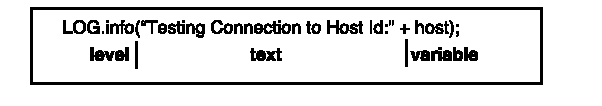
\includegraphics[width=1\columnwidth]{logexample}
	\caption{An example of a logging statement}
	\label{fig:logexample}
\end{figure}




The rich knowledge in logs has lead to the development of many log processing tools such as \textsl{Splunk}~\cite{carasso2012exploring}, \textsl{Xpolog}~\cite{xpolog}, \textsl{Logstash}~\cite{xu2013detecting} and research tools such as Salsa~\cite{TanSalsa}, log-enhancer~\cite{Yuan} and Chukwa~\cite{chukwa} that are designed to analyze logs as well as improve logging statements. However, when logging statements are changed, the associated log processing tools may also need to be updated. For example, Figure~\ref{fig:ExampleOfLogChange_LPA} demonstrates a case in which a developer removes the elapsed time for an event. Removing information from a logging statement can affect log processing tools that rely on the removed information in order to monitor the health of the application. Prior research shows that 60\% of the logging statements that generate output during system execution are changed~\cite{IanWCRE}. Such changes may affect the log processing tools that heavily depend on the logs that are generated by these logging statements.

Knowing whether a logging statement is likely to change in the future is helpful to reduce the effort that is required to maintain log processing tools. If a developer of a log processing tool knows that a logging statement is likely to change, the developer can opt not to depend on the logs that are generated by this logging statement. Instead, the developer can let the log processing tool depend on output generated by logging statements that are likely to remain unchanged. Depending on logging statements that remain unchanged will reduce the maintenance effort that is required for keeping the log processing tool consistent with the ever-changing logs. 

%As changes to logging statements can affect the log processing tools depending on them, it is necessary to identify the cause for these logging statement changes. 

To decide whether a logging statement will change in the future, we must understand which factors play an important role during such a change. The following factors can influence whether a logging statement will change:
\begin{enumerate} 
\item the contents of the logging statement,
\item the location of the logging statement,
\item and the developer who added the logging statement into the source code
\end{enumerate}
In this paper, we examine which of these factors can help to decide whether a logging statement will change. First, we present a preliminary study which was done to get a better understanding of the stability of logging statements in four open source applications namely ActiveMQ, Camel, Cloudstack and Liferay. In this preliminary study, we find that 20\%-45\% of the logging statements are changed at least once during their lifetime in the studied applications. Therefore, developers of log processing tools have to carefully select the logging statements to depend on. 

Second, we explore factors that are important for explaining the stability of a logging statement using a random forest classifier. This classifier uses metrics that describe the three factors mentioned above to decide the likelihood of changing a logging statement.
The most important observations in this paper are:

%We identify three main factors which can cause changes in logging statements namely: 1) who introduces and changes logs, 2) where the logging statement are placed, and 3) what is content of the logged statement.  


% These log changes can affect the log processing tools which heavily depend on them and maintenance cost will be high~\cite{IanWCRE}. 
\begin{figure}[t]
	\centering
	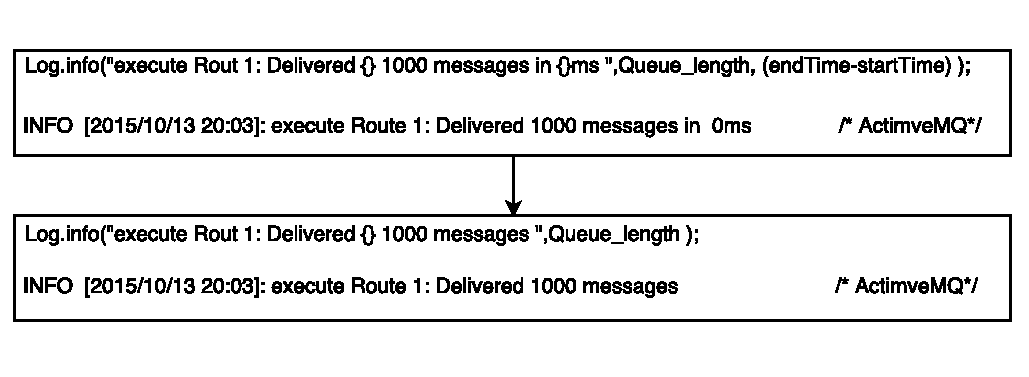
\includegraphics[width=1\columnwidth]{ExampleOfLogChange_LPA}
	\caption{Modification of a logging statement}
	\label{fig:ExampleOfLogChange_LPA}
\end{figure}

\begin{figure*}[t]
	\centering

	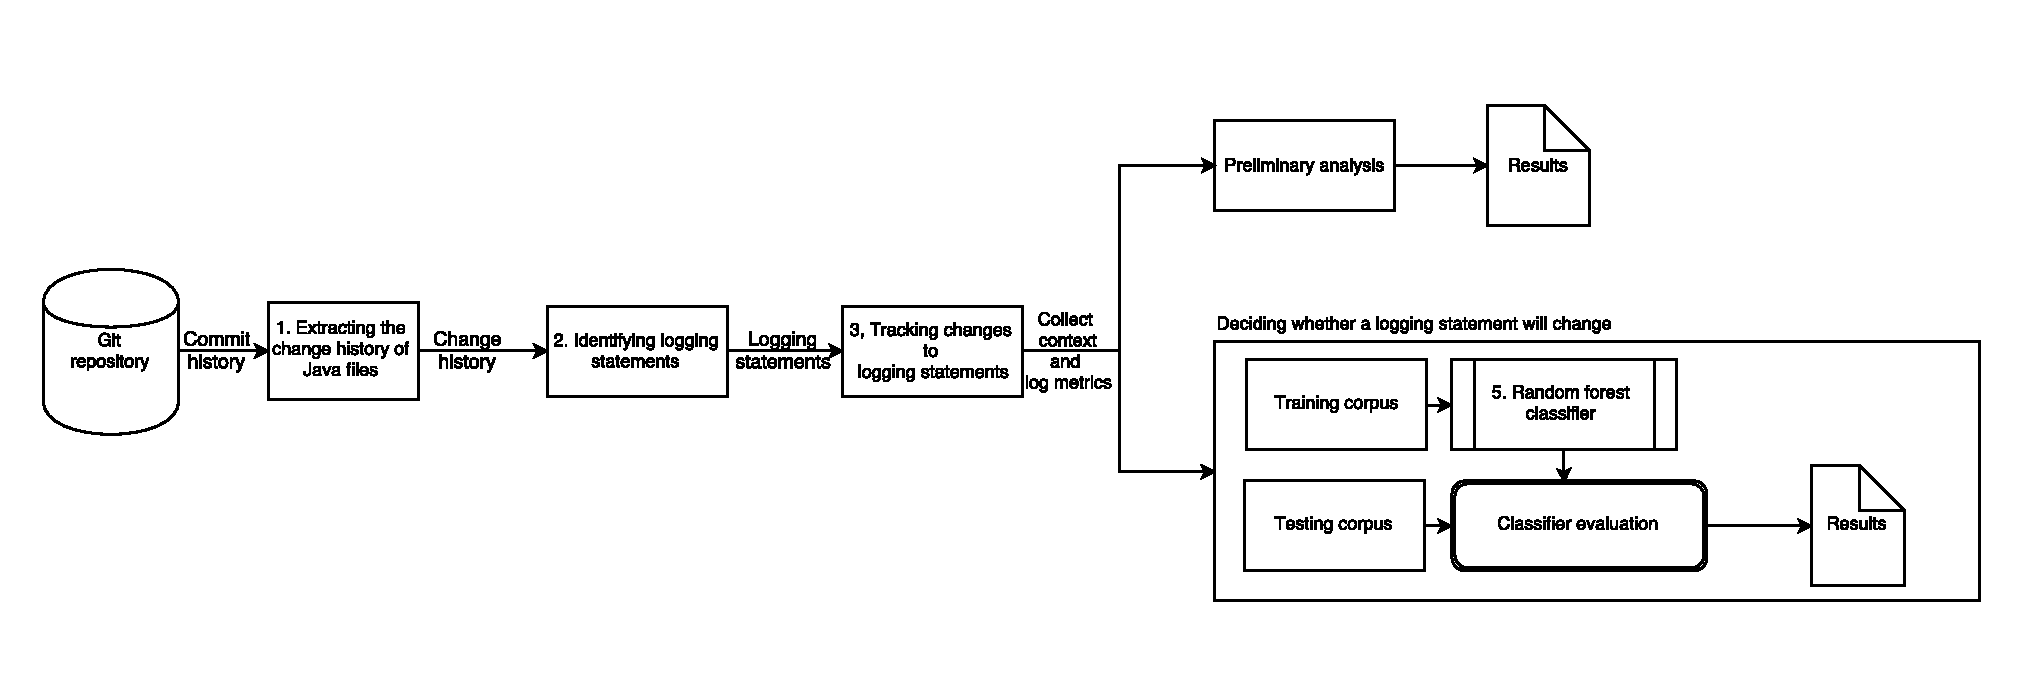
\includegraphics[width=2\columnwidth,
	height=.65\columnwidth,trim={0 1cm 0 1cm },clip]{LogGenalogyMethdology}



	\caption{Overview of the data extraction and empirical study approach}
	\label{fig:LGmethod}
\end{figure*}


%To identify the influence of these factors, in this paper we first study how much logging statements are changed across multiple releases in the four software applications. We find that 35\%-50\% of the logging statements are changed at least once during their lifespan in the studied applications. We also find that a single log changes between 0 to 10 times within its lifetime and can be changed by more than one developer. These results suggest that log processing tools have to be constantly monitored at every release to prevent breakage by the changes to logging statements. 

%To identify which factors the stability of logging statements and model which logs will change in the future, we build a random forest classifier using context and log metrics. The most important observations in this paper are:
\begin{enumerate}
	\item We model whether a logging statement will be changed in the future using a \emph{random forest} classifier with 83\%-91\% precision and 65\%-85\% recall. 
%	Our \textsl{random forest} achieves an precision of 89\%-91\% and recall of 71\%-83\%, when predicting which logs will be changed.


	\item Logging statements that are added by highly experienced developers and very new developers are less likely to be changed. We find that in three of the studied applications the top three developers add more than 60\% of the logging statements and 70\% of the logging statements that are added by the top three developers remain untouched. 
	
	\item Logging statements added by developers who have little ownership on the file that contains the logging statements have a higher likelihood of being changed. We find that 27\%-67\% of all log changes, are done on logging statements added by developers who own less than 20\% of the file.
 
	
%	logging statements added by developers who own less than 20\% of the file are, 1.2-1.6 times more likely to be changed later.
%	 27\%-67\% of all logging statement changes, are done on logging statement added by developers who own less than 20\% of the file. 
	
	
%	\item FIXME Logging statements changed by developers who have less ownership in that file are 0.4-1.4 times more likely to be changed again than logs changed by owners of the file in three of the applications.
%	\item FIXME Developer experience is negatively correlated to log stability in the studied applications, suggesting that logs added by more experienced developers are more stable. This findings suggest that knowledge of the code in a file is important when considering the stability of a logging statement. As a result, maintainers of log processing tools can take special care when importing log statements written by developers who have less experience or with no ownership of the file in which the statement was added.
	\item Large files (i.e., SLOC is 2$\times$-3$\times$ the median) with a low log density are more likely to have changes to their logging statements than well logged files.

%	\item  Change metrics such as SLOC, number of variables logged and number of variables declared are strong predictors of log stability within the studied applications. 

\end{enumerate}

The above findings can assist the maintainers of log processing tools with selecting the logging statements on which they let their tools depend. %importing logging statements to be used by their tools and decrease the maintenance effort.
%
%should be careful when importing log statements written in larger file with less number of logs. 
%
%These log processing tools are used to generate information for capacity planning of large-scale systems~\cite{hassan2008industrial,nagappan2009efficiently}, to monitor system health~\cite{bitincka2010optimizing} or to detect abnormal system behavior~\cite{JiangICSM2008}. These tools rely heavily on the log messages themselves and require continuous maintenance when the format or content of logs are changed.
%
% and use the data to answer the following research questions.
%
%\textbf{RQ1:} \textbf{How much do logs change over time and why do the changes occur?}
%
%Based on our quantitative analysis of the studied systems we identify three categories of change frequency in logs. If a log is changed more than four times we categorize it as \textsl{`Frequently Changed'}, if it has one to three changes, it is categorized as \textsl{`Changed'} and if there are no changes made we categorize it as \textsl{`Never Changed'}. We find that in our studied systems, 20-80\% of the logs are changed at least once throughout their lifespan.
%
%\textbf{RQ2:} \textbf{Can metrics from code, log and developer dimension help in explaining the stability of logs?}
%
%We collect the product and change metrics from three dimensions namely code, log and developer information. Our \textsl{random forest} achieves an accuracy of 89\%-91\% and recall of 71\%-91\%, when predicting which logs have higher likelihood of getting changed. We also identify significant metrics from each of the three dimensions, that affect the stability of logs. We find  developer experience, source lines of code, file ownership, log density in the file are strong predictors in classifying if a log will change in the future. 
%
% Our results show that product and process metrics obtained from code, log and developer information can help in identifying unstable logs in our studied systems. This can help in reducing the effort needed in the maintenance of log processing applications, as system maintainers can flag the logs that have the potential of being changed in subsequent releases and track them. 
% 
The remainder of this paper is organized as follows. Section~\ref{analysis} presents the preliminary analysis that motivates our study. Section~\ref{prediction} describes the random forest classifier and the analysis results. Section~\ref{related} describes the prior research that is related to our work. Section~\ref{threats} discusses the threats to validity. Finally, Section~\ref{conc} concludes the paper.
 
 
% However, as these tools are not scalable for all companies and systems, companies prefer in house development or customization of these tools for their specific purposes. 
\section{Methodology}
\label{Methodology}
In this section we present our rationale for selecting the systems we studied and present our data extraction and analysis approach.


In this paper, we aim to find the unstable logs in a system for easier management of log processing tools. We cloned locally over 15 projects which had more than 10,000 commits in their git repository. We also verify if the projects utilize a bug tracking system like 'JIRA' or `Bugzilla' because, this helps to tag commits to specific development activities (i.e., bug fix, improvement, new-features). We use the `grep' command to recursively search for all log lines within `.java' files in each project in the cloned repositories. We picked the top four projects with the highest log line count. The four open source projects are: Liferay, Camel, ActiveMQ and CloudStack. All studied systems have extensive system logs and Table~\ref{tba:overviewsystems} presents an overview of the systems.

\begin{table}[tbh]
\centering \protect\caption{An overview of all studied systems}


\label{tba:overviewsystems} %
\begin{tabular}{lllll}
\hline 
Projects  & Liferay  & Camel  & ActiveMQ  & CloudStack \tabularnewline
\hline 
Starting release  & 6.1.0-b3  & 1.6.0  & 4.1.1  & 2.1.3 \tabularnewline
End release  &7.0.0-m3  & 2.11.3  & 5.9.0  & 4.2.0 \tabularnewline
Total \# of releases   & 24  & 43  & 19 & 111 \tabularnewline
Total added code  & 3.9M  & 505k  & 261k  & 1.09M \tabularnewline
Total deleted code  & 2.8M  & 174k  & 114k  & 750K \tabularnewline
Total \# added logs  & 10.4k  & 5.1k  & 4.5k  & 24k \tabularnewline
Total \# deleted logs  & 8.1k  & 2.4k  & 2.3k  & 17k \tabularnewline
\hline 
\end{tabular}
\end{table}

\textbf{Liferay}\footnote[1]{http://www.liferay.com/}:  Liferay is a free and open source enterprise project written in Java. It provides platform features which are used in development of websites and portals.
% We select liferay as it is one of the leading platforms for platform development~\cite{LiferayGartner} and has growing user base~\cite{LiferayUser}.
  It also has an extensive issue tracking system in JIRA which helps in categorizing the commits as bug fixes, improvements, . We study the releases from 6.1.0 to 7.0.0-m3 which cover more than three years of development from 2010 to 2014

%Hadoop is an open source software framework for distributed storage and for the processing of big data on clusters. Hadoop uses the MapReduce data-processing paradigm. The logging characteristics of Hadoop have been studied in prior research~\cite{IanWCRE,EMSEIAN,IanContextinformation}. We study the releases from Hadoop 0.20.1 to 2.2.0.


\textbf{Camel}\footnote[2]{http://camel.apache.org/}: Camel is an open source integration platform based on enterprise integration patterns. We analyze Camel release 1.6 to 2.11.3 which cover more than five years of development from 2009 to 2013. 
\begin{figure*}
	\centering
	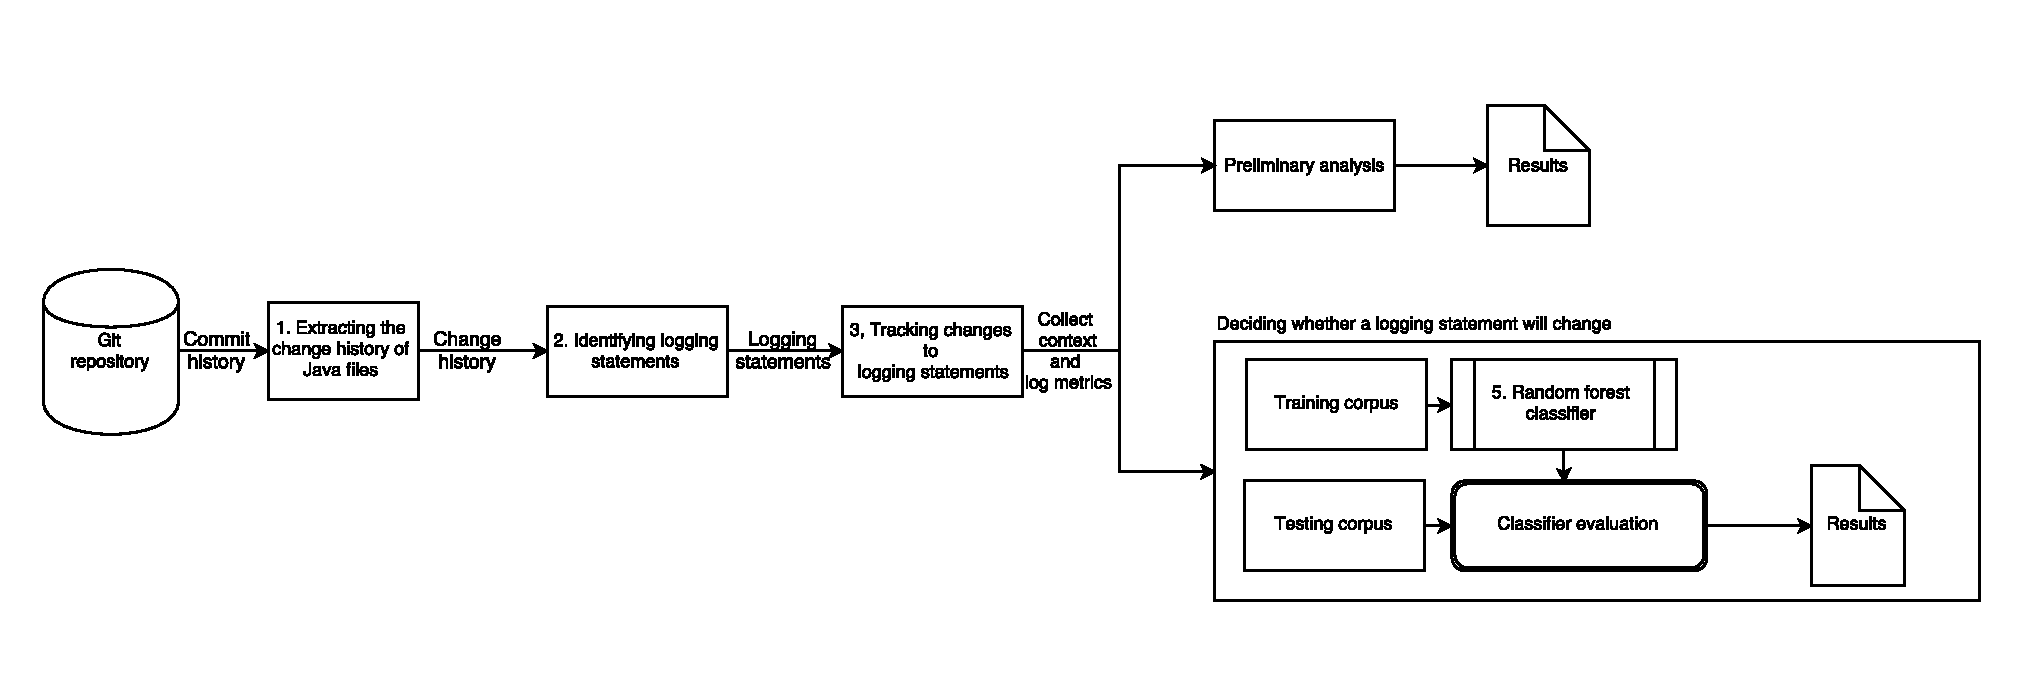
\includegraphics[width=1.7\columnwidth,height=0.50\columnwidth]{LogGenalogyMethdology}
	\caption{Overview of the data extraction and case study approach}
	\label{fig:LGmethod}
\end{figure*}



\textbf{ActiveMQ}\footnote[3]{http://activemq.apache.org/}: ActiveMQ is an open source message broker and integration patterns server. We covered ActiveMQ release 4.1.1 to 5.9.0 which cover more than 6 years of development from 2007 to 2013.


\textbf{CloudStack}\footnote[4]{https://cloudstack.apache.org/}: Apache CloudStack is open source software designed to deploy and manage large networks of virtual machines, as a highly available, highly scalable Infrastructure-as-a-Service (IaaS) cloud computing platform. We covered CloudStack release 2.1.3 to 4.20 which cover more than 3 year of development from 2010 to 2014.


Figure~\ref{fig:LGmethod} shows a general overview of our approach, which consists of four steps: (1) We mine the git repository of each studied system to extract all commits made for each file.(2) We identify the log changes in the extracted files. (3) We track the changes made to each log across the commits. (4) We extract the JIRA issues for the commits and collect the developer metrics when there is a log change in the commit.  We use a statistical tool R~\cite{ihaka1996r}, to perform experiments on the data to answer our research questions. 

\subsection{Study Approach}

 In the reminder of this section we describe the each of these steps.

\subsubsection{Extracting Code Evolution}
In order to find the stability of logs we have to identify all the `Java' files in our studied systems. To achieve this, we clone the \emph{master} branch of the git repository of each studied system locally. We use the `find' command to recursively find all the files which end with pattern `*.java'. To remove the \textsl{Java Test} files, we use `grep' command to filter all files which have `test' or `Test' in their pathname.

 After collecting all the Java files from the four studied systems, we use their git repository to obtain all the changes made to the file within the time-frame discussed above. We use the `follow' option to track the file even when they are renamed or relocated within our studied systems. We flatten all the changes made to files to include the changes made in different branches but exclude the final merging commit. Using this approach, we obtain a complete history of each \emph{Java} file. 

\subsubsection{Identifying Log Changes}
From the extracted code evolution data for each \emph{Java} file, we identify all the log changes made in the commits. To identify the log statements in the source code, we manually sample some commits from each studied system and identify the logging library used to generate the logs. We find that the studied systems use \textsl{Log4j}\footnote{http://logging.apache.org/log4j/2.x/}~\cite{EMSEIAN} and \textsl{Slf4j}\footnote{http://www.slf4j.org/} widely and \textsl{logback}\footnote{http://logback.qos.ch/} sparingly. Using this information we identify the common method invocations that invoke the logging library. For example in  ActiveMQ and Camel a logging library is invoked by method named `LOG' as shown below.
\hypobox{ LOG.debug(``Exception detail", exception);}

In CloudStack it is usually done through `\_logger' as follows.

\hypobox{\_logger.warn(``Timed out: " + buildCommandLine(command));}

As projects can have multiple logging libraries throughout its life-cycle, we use regular expressions to match all the common log invocation patterns (i.e., `LOG',`log',`\_logger',`LOGGER',`Log'). We count every such invocation of a logging library as a log.


\subsubsection{Tracking Log Changes}
After identifying all the log changes made to a file across multiple commits, we track each log individually to find out whether it has changed in subsequent revisions. We first collect all the logs present in a file at the first commit, which form the initial set of logs for the file. Every subsequent commit which has changes to a log appears as an added and deleted log in \textsl{git}. To track these log changes made, we used the Levenshtein ratio~\cite{levenshteinratio}.

To calculate Levenshtein ratio for a pair of added and deleted logs, we first remove the logging method (e.g., LOG) and compare the remaining text. We set a minimum threshold of 0.5 for a pair of added and deleted logs to be considered modified. We set 0.6 because there is atleast 60\% similarity between the pair. We find that when the threshold is set lower there are more false positives and when set higher we miss log modifications. When an added log has levenshtein ratio higher than 0.6 with multiple deleted logs, we consider the pair with highest levenshtein ratio. 

 For example in the logs shown below, we remove the logging method (i.e., LOG) and find that the Levenshtein ratio between the added and deleted pair is 0.86. Hence, this log change is categorized as a log modification.  
 \hypobox{+      LOG.debug(``Call: " +method.getName()+`` took "+ callTime + ``ms");\\ 
 	-        LOG.debug(``Call: " +method.getName()+ `` " + callTime);} 


If the added log does not match any log in our initial set, it is considered as a new log addition and is added to the initial set for tracking in future commits. From this we can track how many times a log is changed and how many commits are made between the changes. 


\subsubsection{Match JIRA to Log Changes}

Using the commit data, we also track the JIRA issues to extract the developer metrics such as developer experience, number of developers involved, issue priority. To achieve this, we extract the JIRA issue IDs from commit messages and use the JIRA repository to extract the JIRA issue. The JIRA issue contains information about the issue such as, type (i.e., bug, improvement, new-feature, task), priority, resolution time and developer information such as number of comments and number of developers involved in the JIRA discussion. We use this information along with code and log churn metrics for answering our research questions. 




 










\section{Study Results}
\label{studyresults}
%In this section, we present our study results by answering our research questions. For each question, we discuss the motivation behind it, the approach to answering it and finally the results obtained. 
%\\
%
%\noindent\textbf{RQ1:} \textbf{How much do logs change over time and why do the changes occur?}
%\\

%\noindent\textbf{Motivation}

%Research has shown that logs evolve along with the code~\cite{IanContextinformation}. When logs are changed, the log  processing tools which are dependent on them also have to get updated. This results in costly maintenance effort. To understand the cost, we have to understand how frequent changes to logs are. Hence, we explore the frequency of changes to logs in our studied systems and why they are changed.\\

%\noindent \textbf{Approach}


%\begin{table*}
%	\centering
%	\caption{Distribution of log changes in different projects}
%	\label{tba:logchangeDistribution}
%	\begin{tabular}{l|>{\centering}p{.1\columnwidth}>{\centering}p{.01\columnwidth} 
%			p{0.01\columnwidth} }
%		\cline{1-4}  	\multicolumn{1}{|c}{Projects}    & \multicolumn{1}{|c}{Never Changed (\%) }  &  \multicolumn{1}{|c}{Changed (\%) }	   &  \multicolumn{1}{|c}{Frequently Changed (\%) }\\ \cline{1-4}   
%		
%		Life Ray      & 78.67     & 19.66 & 1.66           \\
%		
%		Camel      & 55.43    & 37.32 & 7.25            \\
%		ActiveMq   & 34.78     & 62.02 & 3.20           \\
%		CloudStack & 19.68     & 68.61 & 11.71          \\ \cline{1-4}
%	\end{tabular}
%\end{table*}

%\begin{table*}
%	\centering
%	\caption{Distribution of log changes in different projects}
%	\label{tba:logtype}
%	\begin{tabular}{l|llll}
%		\cline{1-5}  	\multicolumn{1}{|c}{Projects}    & \multicolumn{1}{|c}{ ActiveMQ }  &  \multicolumn{1}{|c}{ Camel}	   &  \multicolumn{1}{|c}{ Cloudstack }  & 
%		\multicolumn{1}{|c|}{ Liferay } \\ \cline{1-5}   
%		
%		Log relocation (\%)       & 20.05     & 20.80 &  53.32  & 49.42         \\
%		
%		Log text change (\%)      & 26.59    & 26.37 & 15.54    & 32.70       \\
%		Log variable change (\%)   & 53.18     & 52.75 & 31.08 &  16.75     \\
%		Change of log level (\%) & 0.18   & 0.08 & 0.04  &  1.13       \\ 
%%		Text and variable change (\%) & 2.33     & 6.39 & 22.0   &  30.59    \\ 
%\cline{1-5}
%	\end{tabular}
%\end{table*}


%In this paper we aim to get a better understanding of the
%unstable logs in an project so that we can improve the maintenance of log processing tools. 
In this paper we study the changes that are made to logs across multiple releases in open source projects. The goal of our study is to present a model for deciding whether a logging statement is likely to change in the future. This model can assist developers of log processing tools to decide on which logging statements they want their tool to depend. %In order to understand and build a random forest classifier to predict log changes, it is necessary to identify the extent logs are changed within these projects.
First, we perform a preliminary analysis, in which we examine how often logging statements change, to motivate our work. In this section, we present our rationale for selecting the projects that we studied and present the results of our preliminary analysis of the four studied projects. 

\subsection{Studied Projects}
In this paper, we examine the logging statements in open source projects. We selected these projects based on the following three criteria:
\begin{itemize}
	\item \textbf{Log usage} - The selected projects must make extensive use of logs in their source code
	%	This helps to improve the performace of the random forest classifier and to identify the factors which effect log stability.
	\item \textbf{Project activity} - The projects must have a mature development history (i.e., more than 10,000 commits)
	\item \textbf{Technology used} - To simplify the implementation of our study, we opted to select only projects that are written in Java and are available on a Git repository
%	We pick projects written in Java as it is one of the most popular languages today~\cite{Javaprog}.
%	 to identify and track the log changes across multiple releases. 
\end{itemize}

To select projects matching these criteria, we first selected all Java projects from the list of Apache Foundation Git repositories\footnote{\url{https://git.apache.org/}} that have more than 10,000 commits. Next, we counted the number of logging statements in all \code{*.java} files in a repository using the \code{grep} command in Listing~\ref{lst:grep}.

\vspace{-5mm}
\begin{Code}
\begin{lstlisting}[caption={Counting logging statements}, label={lst:grep}]
grep -icR 
"\(log\.*\)\.\(|info\|trace\|debug\|error\|warn\)(" . 
| grep "\.java"
\end{lstlisting}
\end{Code}
\vspace{-5mm}

This command counts the occurrences in a file of an invocation of a logging library (e.g., \code{log} or \code{\_logger}) followed by the specification of a log level. We sum the occurrences in all files of a project to get the total number of logging statements shown in Table~\ref{tba:overviewsystems}.
%To find the log usage in an project we use the \emph{grep} command to search all lines of code within the \emph{.java} files. %Next, using \emph{git log} we find the total number of commits in the code repositories and select projects which have more than 10,000 commits.
 
We select the four projects (ActiveMQ, Camel, Cloudstack and Liferay) with the highest number of logging statements for further analysis. ActiveMQ\footnote{\url{http://activemq.apache.org/}} is an open source message broker and integration patterns server. Camel\footnote{\url{http://camel.apache.org/}} is an open source integration platform based on enterprise integration patterns. CloudStack\footnote{\url{https://cloudstack.apache.org/}} is an open source project designed to deploy and manage large networks of virtual machines. Liferay\footnote{\url{http://www.liferay.com/}} is an open source platform for building websites and web portals. Table~\ref{tba:overviewsystems} presents an overview of the studied projects. %We pick the releases after incubation for each project, as during incubation the projects might not be used by log processing tools.  


\begin{table}[tb]
	\centering \protect\protect\caption{An overview of the studied projects (all metrics calculated using the latest HEAD of the repository) \cp{FIXME}}
	\smaller
	
	\label{tba:overviewsystems} %
	\begin{tabular}{lrrrr}
		\toprule 
		~ & \textbf{ActiveMQ}  & \textbf{Camel}  & \textbf{CloudStack}  & \textbf{Liferay} \\
		\midrule
		Logging statements & 5.1k  & 6.1k  & 9.6k  & 1.8k \\
		Commits &	 ?  & ?  & ?  & ? \\	
		Months in repository &	 ?  & ?  & ?  & ? \\
%		\# of releases  & 19  & 43  & 111  & 24 \\
		\midrule
		Added lines of code  & 261k  & 505k  & 1.09M  & 3.9M \\
		Deleted lines of code  & 114k  & 174k  & 750k  & 2.8M \\
		Added logging statements  & 4.5k  & 5.1k  & 24k  & 10.4k \\
		Deleted logging statements  & 2.3k & 2.4k  & 17k  & 8.1k \\
		Logging-related changes & 1.8\% & 1.1\% & 2.3\% & 0.3\% \\
		\bottomrule 
	\end{tabular}
\end{table}

\subsection{Data Extraction Approach}

The data extraction approach from the four studied projects consists of three steps, which will be explained further in this section: 

\begin{enumerate}
\item We clone the Git repository of each studied project in order to extract the change history of each file 
\item We identify the logging statements in the repository%, and use the change history to identify changes made to these logging statements
\item We track the changes that are made to each logging statement across commits 
\end{enumerate}

We use R~\cite{ihaka1996r}, to perform experiments and answer our preliminary analysis. Figure~\ref{fig:LGmethod} shows a general overview of our approach and we detail below each of the aforementioned steps. 

\subsubsection*{B.1. Extracting the change history of Java files} 
%In order to find the stability of logs, we have to identify all the Java files in our studied projects. To achieve this, we use the \emph{grep} command to search for all the \emph{*.java} files in the cloned repositories and we exclude the \emph{test} files. 
To examine the changes made to logging statements, we must first obtain a complete history of each Java file in the latest version of the main branch.
We collect all the Java files in the four studied projects and we use their Git repositories to obtain all the changes that are made to the files. We use Git's \emph{follow} option to track a file even when it is renamed or relocated. We include only the changes to logging statements that are made in the main branch as other logging statements are unlikely to affect log processing tools. %We use the \emph{--no-merges} option to flatten the changes to a file and exclude the final merging commit. 

\subsubsection*{B.2. Identifying logging statements}
From the extracted change history of each Java file, we identify all the logging statements.
First, we manually examine the documentation of each studied project to identify the logging library used to generate the logs. %We examine commits rather than code because a project may use multiple logging libraries during its lifetime. 
We find that the studied projects use \textsl{Log4j}~\cite{EMSEIAN}, \emph{Slf4j}\footnote{\url{http://www.slf4j.org/}} and \emph{logback}\footnote{\url{http://logback.qos.ch/}}.
Using this information, we manually identify the common method invocations that invoke the logging library. For example, in ActiveMQ and Camel, a logging library is invoked by a method named \emph{LOG} as shown below.

\hypobox{ LOG.debug(``Exception detail", exception);}

As a project can use multiple logging libraries throughout its lifetime, we use regular expressions to search for all the common log invocation patterns (i.e., \emph{LOG, log, \_logger, LOGGER, Log}). We identify every successful match of this regular expression that is followed by a log level (\emph{info, trace, debug, error, warn}) as a logging statement.


\subsubsection*{B.3. Tracking changes to logging statements}
After identifying all the logging statements, we track the changes made to these statements after their introduction. We extract the change information from the Git commits, which show a \emph{diff} of added and removed code. To distinguish between a change in which a new logging statement is added and a change to an existing logging statement, we must track the changes made to a logging statement starting from the first project commit. Because there may be multiple changes to logging statements in a commit, we must decide to which existing logging statement a change maps.

We first collect all the logging statements in the initial project commit as the initial set of logging statements. Then, we analyze the next commit to find changes to logging statements until we reach the latest commit in the repository. To distinguish between added, deleted and changed logging statements and to map the change to an existing logging statement, we use the Levenshtein ratio~\cite{levenshteinratio}. 

We use the Levenshtein ratio instead of string comparison, because Levenshtein ratio quantifies the difference between the strings on a continuous scale between 0 and 1 (the more similar the strings are, the closer the ratio approaches 1). This continuous scale is necessary to decide between multiple logging statements which can have a similar match to a change. Selecting the best matching logging statement is demonstrated by the example in Listing~\ref{lst:multiplelogs}. In this example, there are two changes made to logging statements: one change and one addition. 

%\hypobox{-        LOG.debug(``Call: " +method.getName()+ `` " + callTime);\\
%	+      LOG.debug(``Call: " +method.getName()+`` took "+ callTime + ``ms"); \space  \space  \space  \space  \space  \space -- \textbf{(a1)}\\ 
%	+      LOG.debug(``Call: " +method.setName()+`` took "+ callTime + ``ms");\space  \space  \space  \space  \space  \space -- \textbf{(a2)}} 

%\begin{Code}
\begin{lstlisting}[caption={Selecting the best matching logging statement}, label={lst:multiplelogs}, float=*]
-      LOG.debug("Call: " +method.getName()+ " " + callTime);
+      LOG.debug("Call: " +method.getName()+ " took "+ callTime + "ms"); // (Statement a1)
+      LOG.debug("Call: " +method.setName()+ " took "+ callTime + "ms"); // (Statement a2)
\end{lstlisting}
%\end{Code}


%within the range 0 to 1 (more similar the strings the ratio approaches 1).

%To calculate Levenshtein ratio for a pair of added and deleted logs, we first remove the logging method (e.g., LOG) and compare the remaining text to increase the accuracy of categorization. 


%We set a minimum threshold of 0.6 for a pair of added and deleted logs to be considered modified. We set 0.6 because there is atleast 60\% similarity between the pair. We find that when the threshold is set lower there are more false positives and when set higher we miss log modifications. When an added log has levenshtein ratio higher than 0.6 with multiple deleted logs, we consider the pair with highest levenshtein ratio. 
To identify the change we calculate the Levenshtein ratio between each deleted and all the added logging statements and select the pair which has the highest Levenshtein ratio. This calculation is done iteratively to find all the changes within a commit. In our example, we find that the Levenshtein ratio between the deleted statement and statement \emph{a1} is 0.86 and between the deleted statement and statement \emph{a2} 0.76. Hence, we consider \emph{a1} as a change. If there are no more deleted logging statements, \emph{a2} is considered a newly added instead of a changed logging statement. 

We extend the initial set of logging statements with every newly added logging statement. 
%Using the above process, we decide when a logging statement added into a file and the log is added to the initial set for tracking in future commits. From this, we track how many times a log is changed and how many commits are made between the changes. 
As we do not have change information for logging statements which are added near the end of the lifetime of the repository, we exclude these logging statements from our analysis. We find that in the studied projects, the maximum number of commits between the addition of a logging statement and its first change is 390, as shown in Table~\ref{tba:summaryofnewLogchange}. We exclude all logs added to the project 390 commits before the last commit of our analysis. 


%, we find that this varies widely within the project between 37 to 390 commits. To eliminate such logs, we use the maximum number of commits before a newly added log is changed within the studied projects and exclude all new logs added before that many commits from our analysis.  



%\subsubsection{Match JIRA to Log Changes}

%\subsection{Metric analysis}
%After collecting all the log changes, we look at the different types of log changed which occur in our studied projects. We find that log relocation occurs more often than other types of log changes in all of the studied projects. We find that log relocation occurs between 20\%-50\% as seen in Table~\ref{tba:logtype}. As log relocations have no changes to the text or variables in logs, their effect on log processing tools is limited. Hence we exclude log relocation changes from our datasets and non-relocation changes for the random forest classifier. 




%To achieve this, we clone the \emph{master} branch of the git repository of each studied project locally. We use the `find' command to recursively find all the files which end with pattern `*.java'. To remove the \textsl{Java Test} files, we use the `grep' command to filter all files which have `test' or `Test' in their pathname.

%Figure~\ref{fig:LGmethod} shows a general overview of our approach, which consists of five steps: (1) We mine the git repository of each studied project to extract all commits made for each file.(2) We identify the log changes in the extracted files. (3) We track the changes made to each log across the commits. (4) We categorize the log changes in the commit and collect the process and change metrics for each log change in the commit. We use R~\cite{ihaka1996r}, to perform experiments and answer our preliminary analysis and case study.  


%Camel, CloudStack  and Liferay. Table~\ref{tba:overviewsystems} presents an overview of the projects.

%{ActiveMQ}



%Prior to performing our case study, we perform a preliminary analysis to evaluate how much logs change in the four studied projects.
%present the results of our preliminary analysis on the log changes in the four studied systems. 
%\subsection{Approach}
%\noindent \textsl{Approach\\}\\
%Using the tracked log changes, we look at how many times a single log can change in its lifetime. We use the tracked log data from Section~\ref{Methodology} to find the frequency of log changes in the studied projects. 



%Next, we look how many times can a single log change it its lifetime. 


%\begin{figure}[tb]
%	\centering
%%	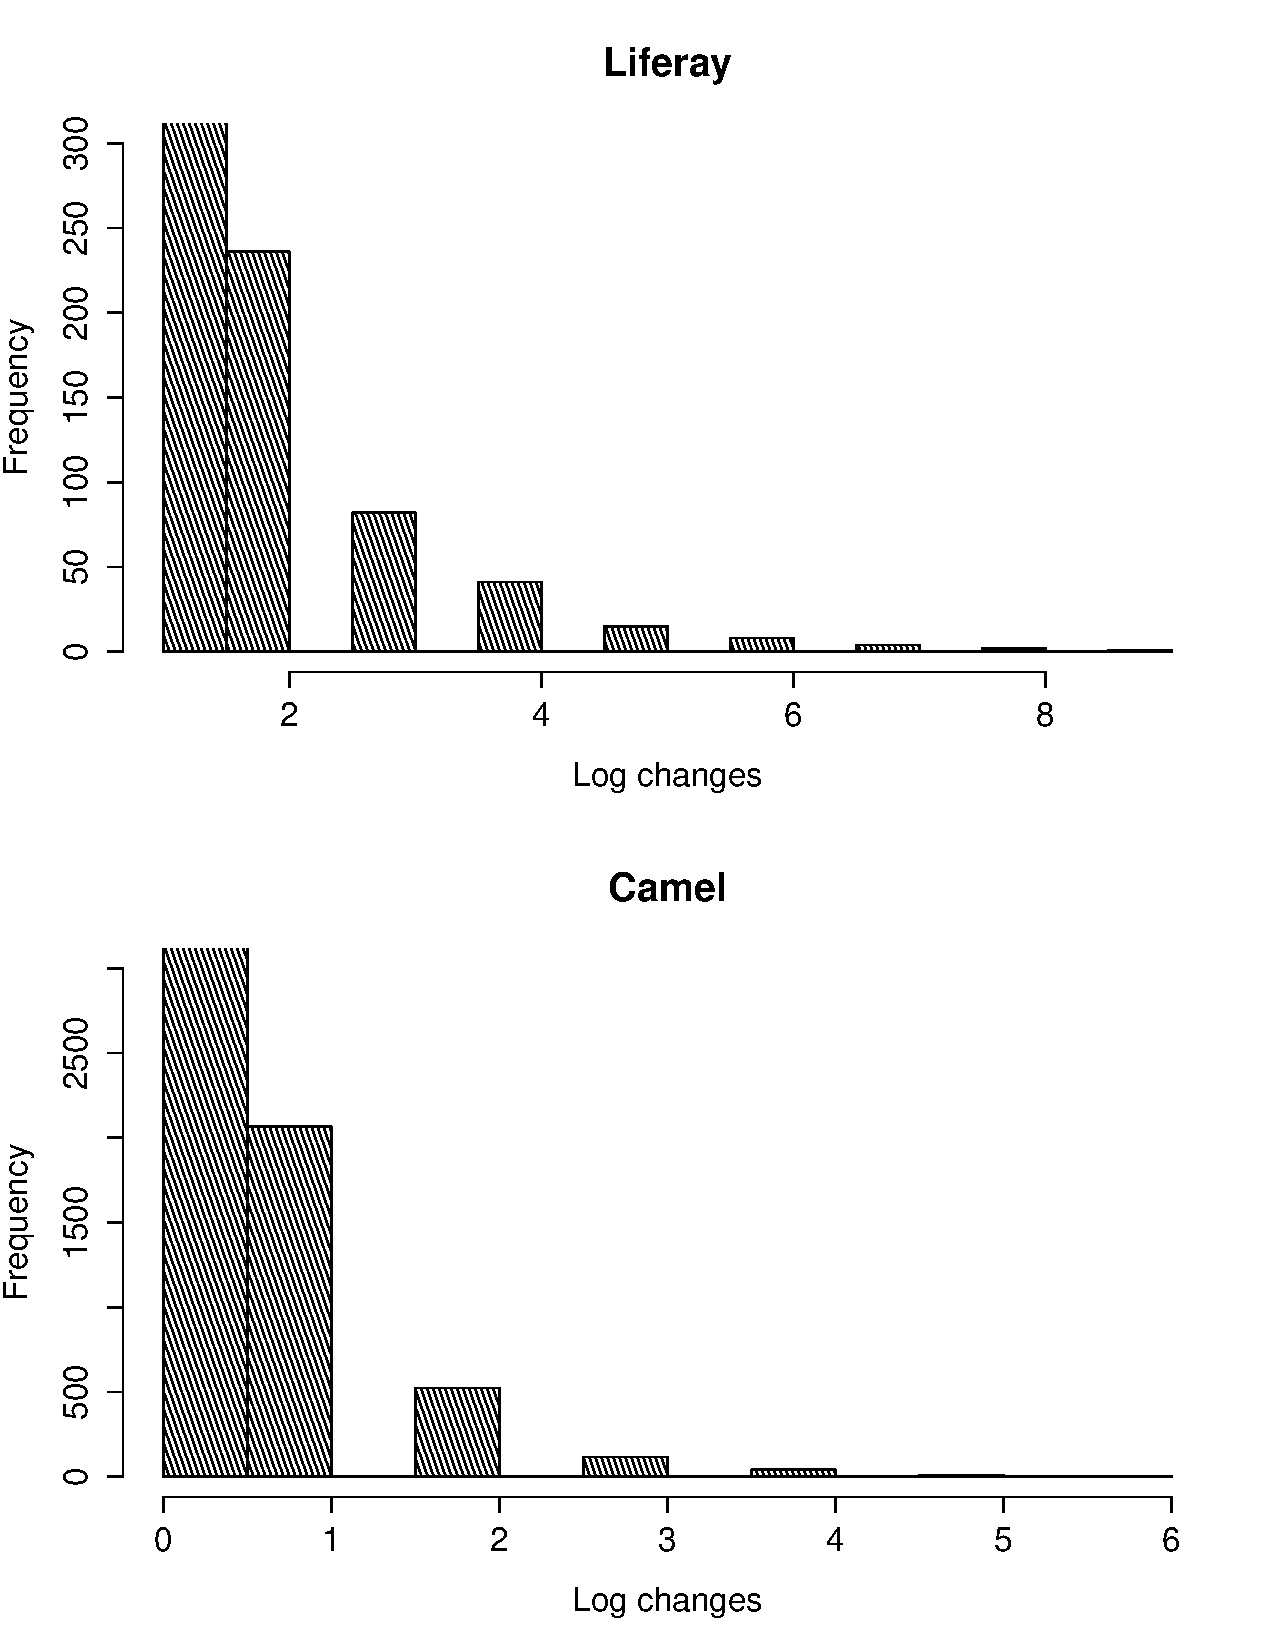
\includegraphics[width=0.7\linewidth]{RQ1_Liferay_Camel_Logchangefreq}
%	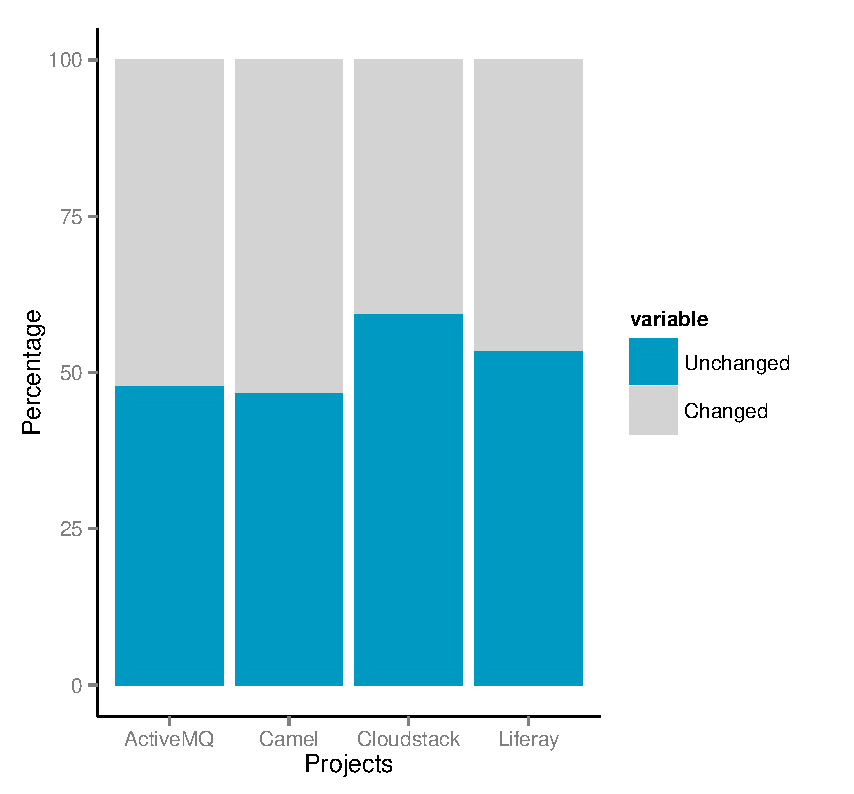
\includegraphics[width=0\linewidth]{Percentageofchanges}
%	\caption{Percentage of log changes in the studied projects.}
%	\label{fig:RQ1_Liferay_Camel_Logchangefreq}
%\end{figure}

\begin{figure}[tb]
	
	\centering
%	\captionsetup{justification=centre}
	
%		\subfloat[Percentage of log changes]{\includegraphics[width=0.5\linewidth]
%			{Percentageofchanges}\label{fig:percentage} }

	\subfloat{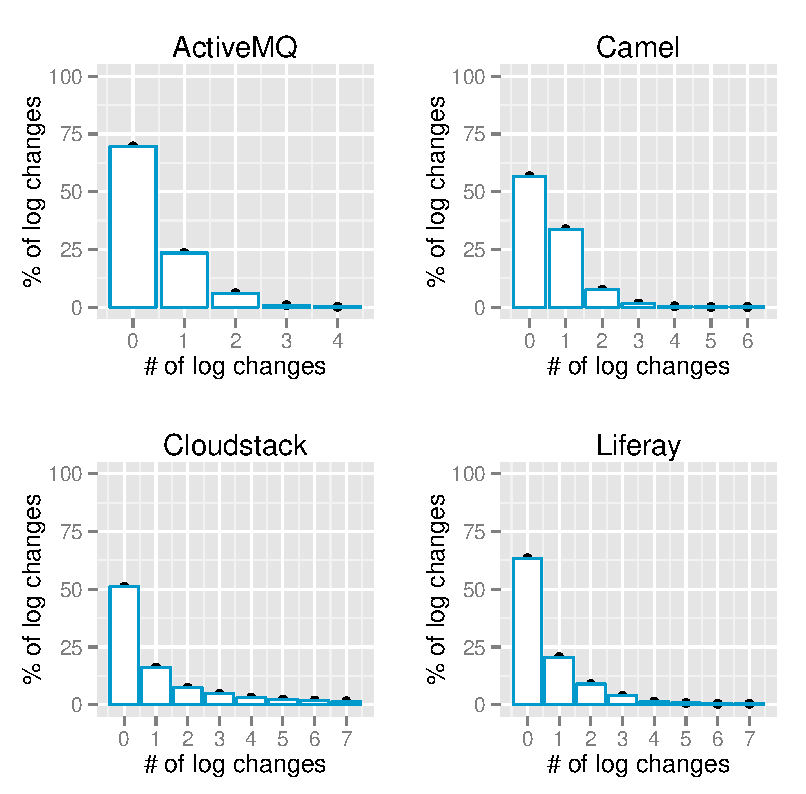
\includegraphics[width=1\linewidth]
		{frequencyofLogchanges}\label{fig:Feq} }
	
	%	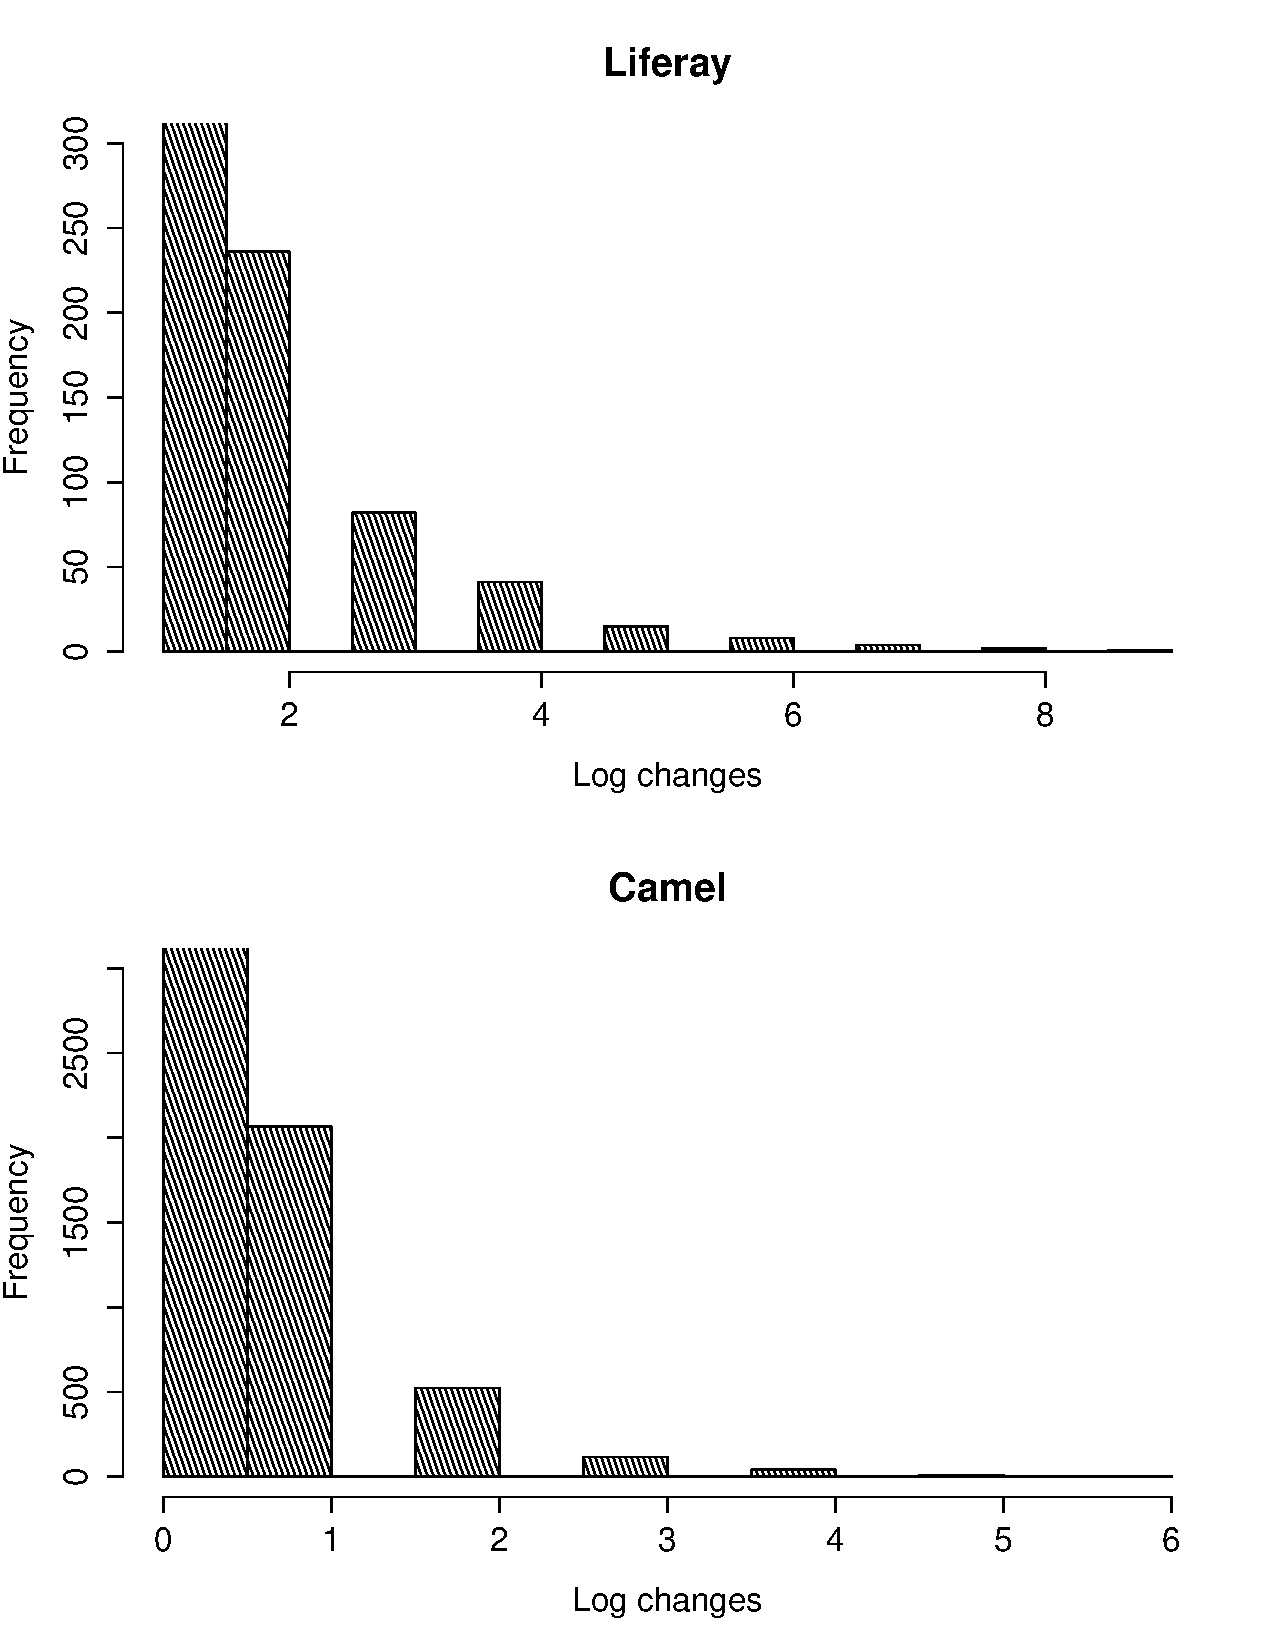
\includegraphics[width=0.7\linewidth]{RQ1_Liferay_Camel_Logchangefreq}
%	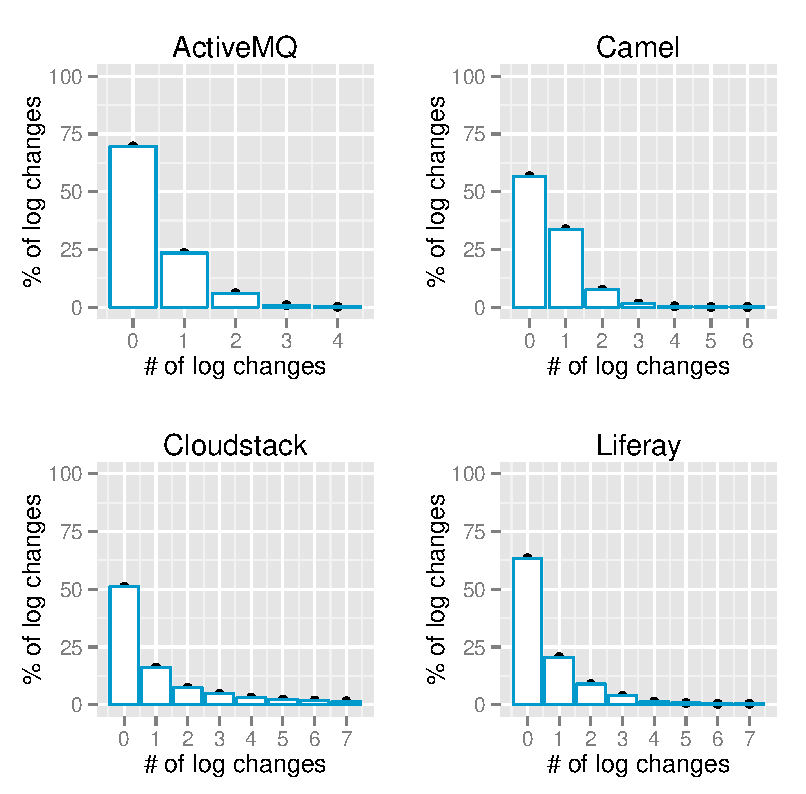
\includegraphics[width=0.9\linewidth]{frequencyofLogchanges}
	\caption{Distribution of log changes in the studied projects	} 
	\label{fig:frequencyofLogchanges}
\end{figure}



%To find how frequently logs change, we conduct a quantitative analysis on the studied systems. We use the tracked log data for each studied system as explained in Section~\ref{Methodology}. From each project, we select a random sample with 95\% confidence interval. We follow the same iterative process as in prior research~\cite{IanIcesm} to find how frequently logs change in our studied systems. 





%\begin{figure}[tb]
%	
%	\centering
%	%	\subfloat{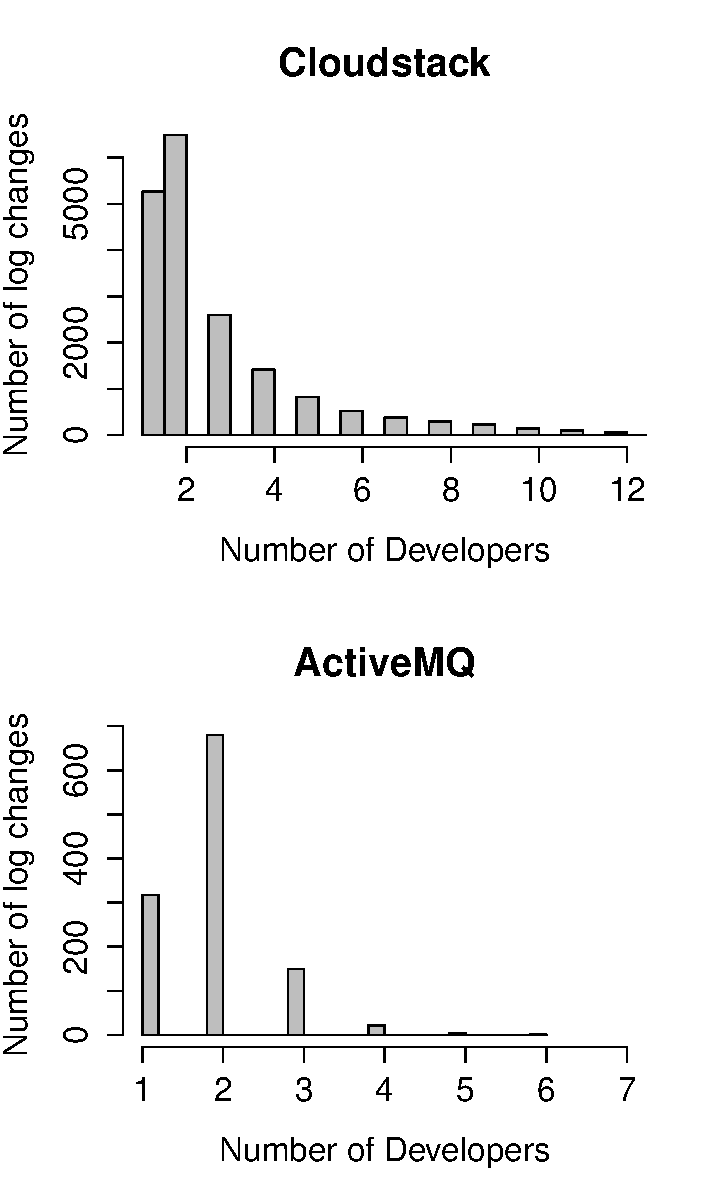
\includegraphics[width=0.5\linewidth]{CA_numberofDevelopers}\label{fig:f1}}
%	%	\hfill
%	\subfloat{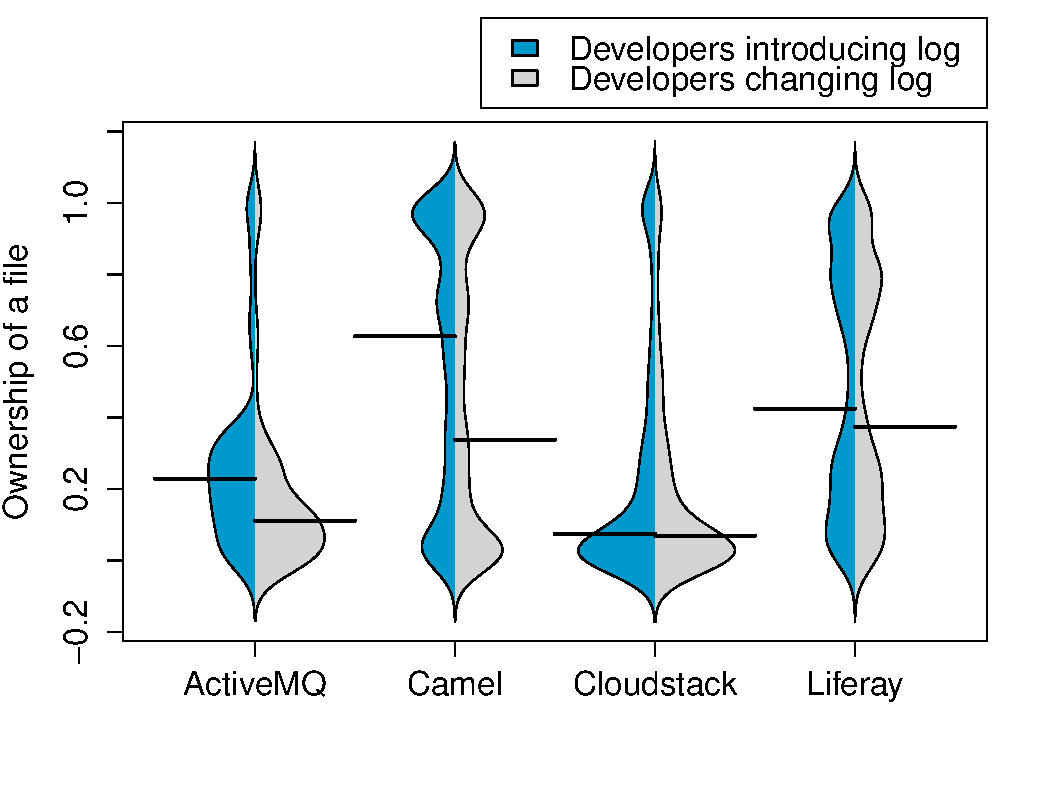
\includegraphics[width=1\linewidth]{ChangedvsChangesorNot}\label{fig:f2}}
%	\caption{Distribution of file ownership against developers introducing the log vs developers changing the log.}
%	\label{fig:ChangedvsChangesorNot}
%\end{figure}



%\begin{figure}[tb]
%	
%	\centering
%	%	\subfloat{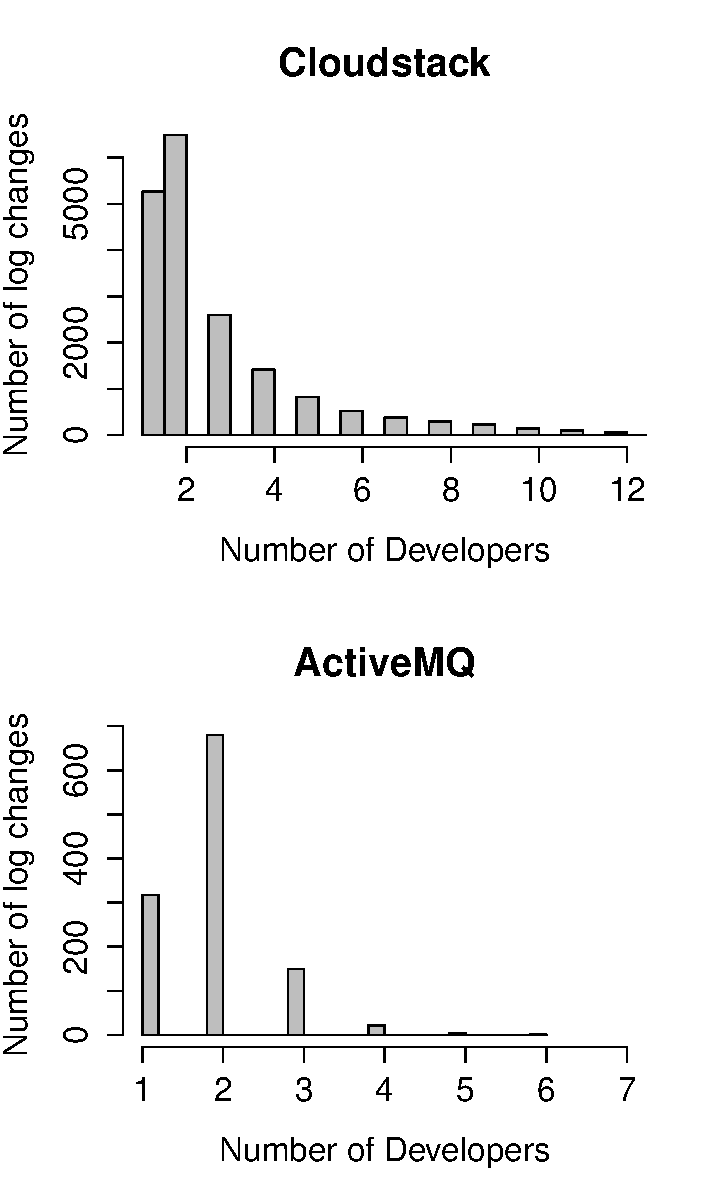
\includegraphics[width=0.5\linewidth]{CA_numberofDevelopers}\label{fig:f1}}
%	%	\hfill
%	\subfloat{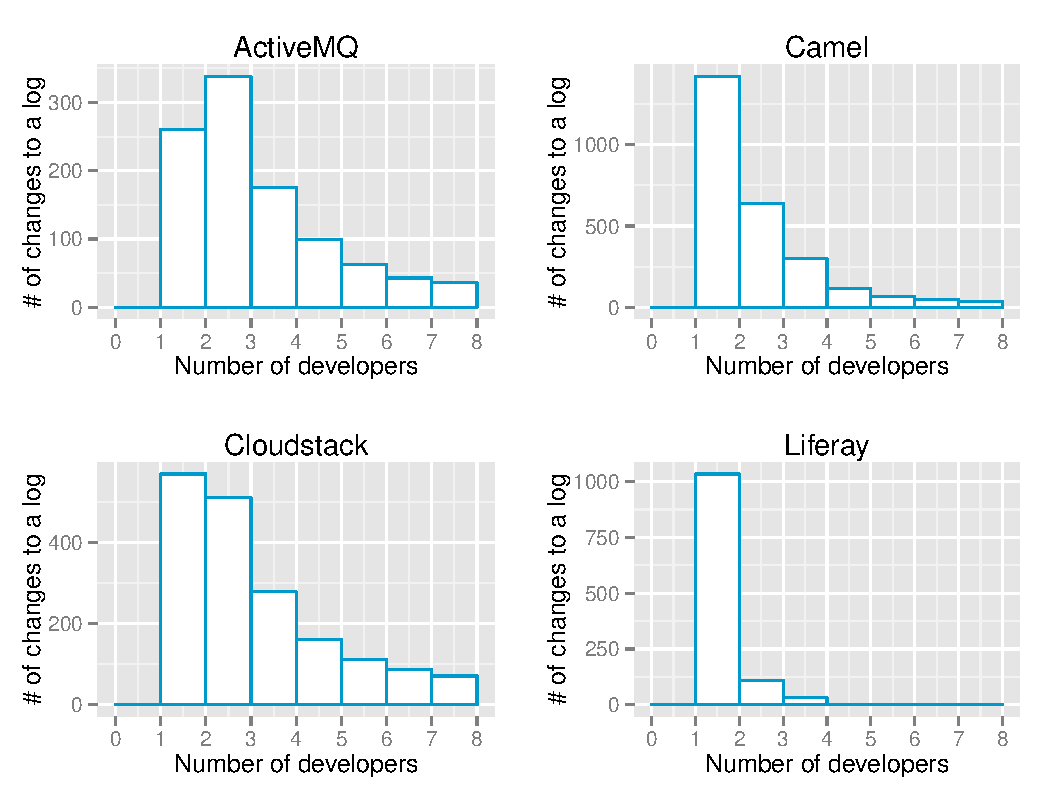
\includegraphics[width=1\linewidth]{NumberofDevelopers}\label{fig:f2}}
%	\caption{Distribution of the number of developers responsible
%		for changing a log.}
%	\label{fig:NumberofDevelopers}
%\end{figure}





\subsection{Results \cp{FIXME}}

\begin{table}[tb]
	\centering
	\smaller
	\caption{The number of commits before a newly added log is changed in the studied projects \cp{BOXPLOTS}}
	
	\begin{tabular}{lrrrrrr}
		\toprule
		\textbf{Project} & \textbf{Min} & \textbf{1st Qu} & \textbf{Median} & \textbf{Mean} & \textbf{3rd Qu} & \textbf{Max} \\
		\midrule
		ActiveMQ   & 1   & 2      & 7      & 9    & 14     & 37  \\
		Camel      & 1   & 1      & 2      & 4    & 5      & 117 \\
		Cloudstack & 1   & 1      & 3      & 17   & 14     & 390 \\
		Liferay    & 1   & 1      & 1      & 7    & 1      & 130\\
		\bottomrule
	\end{tabular}
	\label{tba:summaryofnewLogchange}
\end{table}


%\subsubsection*{C.1. Change frequency}
\hypobox {Developers change 35\%-50\% of the logs across our studied projects. }
Figure~\ref{fig:frequencyofLogchanges} shows the percentage values for the number of times a log is changed in each of the studied projects. This shows that logs change extensively throughout the lifetime of an project which can affect the log processing tools.

\begin{table}[t]
	\centering
	\smaller
	\caption{Total code churn in the commits where a newly added log is changed \cp{BOXPLOTS}}
	
	\begin{tabular}{lrrrrrr}
		\toprule
		\textbf{Project} & \textbf{Min} & \textbf{1st Qu} & \textbf{Median} & \textbf{Mean} & \textbf{3rd Qu} & \textbf{Max} \\
		\midrule
		ActiveMQ   & 2  & 25      & 47     & 141    & 163     & 493  \\
		Camel      & 2   & 13      & 32      & 98    & 133      & 456 \\
		Cloudstack & 2   & 66      & 234      & 410   & 574     & 4121 \\
		Liferay    & 2   & 6      & 14     & 28    & 27     & 278\\	
		\bottomrule
		
	\end{tabular}
	\label{tba:summaryofnewLogCodechange}
\end{table}




\textbf{75\% of the new logs which change, are changed within 15 commits since their addition.} From Table~\ref{tba:summaryofnewLogchange}, we find that majority, i.e., 75\% are changed within 15 commits since addition.  We also find that the median code churn during these log changes is less than 50 lines of code in three of the studied projects as seen in Table~\ref{tba:summaryofnewLogCodechange}. This suggests that the log changes are more likely to be changed due to rewording changes rather than major changes to the added feature. This means that new logs which are introduced prior to 15 commits in the studied projects, are less likely to break the log processing tools which might depend on them. 


%\textbf{25\% of the new logs which change, are changed after 15 commits since their addition.} From Table~\ref{tba:summaryofnewLogchange}, we find 25\% of the new logs added are changed after 15 commits since their addition. We also find that the code churn during these log changes is more than 150 lines of code in three of the studied projects as seen in Table~\ref{tba:summaryofnewLogCodechange}. This suggests that these log changes are more likely to be changes to the feature rather than rewording changes, and are more likely to affect the log processing tools. 

%This also means that the remaining 25\% of log changes might break the log processing tools which might rely on them, as they are changed much later. 



%rewording or after-thoughts rather than change of feature.

% This short time between addition and log change suggests that log change are more likely to be rewording or after-thoughts rather than change of feature. This is seen in Table~\ref{tba:summaryofnewLogCodechange} where in three of the projects, the code churn is less than 50 lines of code for 50\% of the new logs which are changed before 15 commits since addition. 



%We find that logs are added throughout the lifetime of an project and these logs are changed within 

%, the logs added near the end of our study time-frame can change but will not be considered in our analysis. We find that a new log is changed between 37 to 390 commits within our projects as seen in Table~\ref{tba:summaryofnewLogchange}. To eliminate such logs, we find the maximum number of commits before a newly added log is changed within the studied projects and exclude all new logs added before that many commits from our analysis. 


%From Table~\ref{tba:summaryofnewLogchange}, we see that the maximum value varies greatly within the studied projects and we exclude all newly added logs into the project before the 
 
%as shown in Figure~\ref{fig:RQ1_Liferay_Camel_Logchangefreq}. 



%Based on frequency of changes, we categorize logs into 3 categories namely: a) Frequently Changed, b) Changed and c) Never Changed as shown in Table~\ref{tba:logchangeDistribution}. If a log is changed more than four times it is categorized as `Frequently Changed'. If it is changed 1 to 3 times it is categorized under `Changed' and if it did not change it is categorized under `Never Changed'. We select four as the threshold as we observe that majority of logs only have 1 to 2 changes as seen in Figure~\ref{fig:RQ1_Liferay_Camel_Logchangefreq}. We see that the majority of logs never change in Liferay and the majority of logs in ActiveMQ and CloudStack are changed atleast once. This may be because Liferay has fewer logs per source code file (i.e., lower log density) when compared to ActiveMQ and CloudStack as seen in Table~\ref{tba:overviewsystems}. 


%\subsubsection*{C.2. Developer impact}
%After identifying the frequency of changes within the studied projects, we find the number of the developers responsible for the log changes and also if they own the file which contains the log. We use the developer name available from the `git log' to count the number of developers who change a log. To decide whether a developer owns a file we calculate the ratio of number of lines written by him to the total lines of code using the `blame' command available in Git. Since \emph{blame} only shows the changes made to a file in the last commit, to calculate the contribution of a developer to a file we recursively look at changes made in previous commits by that developer. We use the \emph{blame} to calculate the contribution at each commit and take the mean contribution across all commits to find his ownership of a file.

%we obtain all the the commits made to a file and calculate th



%\hypobox{Logs which change are introduced by developers who have little ownership over the file.} 
%Figure~\ref{fig:ChangedvsUnchangedlogs} shows that in Camel, Cloudstack and Liferay, the logs which change are more likely to be introduced by developers who have less ownership on the files, than logs which are never changed. This suggests that logs can be introduced by non-owners of a file, which leads to logs being changed later. 

%We see that logs are changed by developers who have lesser ownership over the 
%file than the developers who introduce the log.

%We see thats logs are also changed by developers who have lesser ownership than the ones introducing them. Figure~\ref{fig:ChangedvsChangesorNot} shows that in all the studied projects the logs are more likely to be changed by developers who have lesser ownership on the file than the developers who introduce the log. These results suggest that logs are readily changed by developers who access the file but do not have strong ownership characteristics.   



%These results suggest that logs are readily changed by developers who access the file but do not have strong ownership characteristics.

%Figure~\ref{fig:ChangedvsChangesorNot} shows that in all the studied


 

% which change are introduced by developers who have less ownership on files than the developers who introduce the log.
 
%  We also find that in one of the studied projects the majority of logs are changed by two or more developers as seen in Figure~\ref{fig:NumberofDevelopers}. 

% we see that in two of the studied systems, a single developer is responsible for majority of the log changes. 

%This suggests that logs can be 
% do not have strong ownership characteristics and can be changed by developers than one introducing the logs.

%\hypobox {45\%-55\% of the logs are changed atleast once in the studied projects. We find that over 51\% of the changes are made to the static content, variable content and log level. We also find that logs are changed by developers who have little ownership of the file and in two of the projects we find the majority of logs are changed by two or more developers.}

%When logs are changed, they can be changed in five possible ways namely:
%\begin{enumerate}
%	
%	\item { \textbf{Log relocation:} } The log is kept intact but moved to a different location in the file because of context changes (code around the log is changed).
%	
%	\item \textbf{Text change:} The text (i.e., static content) of log is changed. 
%	
%	\item\textbf{Variable change:} One or more variables in the log are changed (added, deleted or modified).
%	
%	\item \textbf{Change of log level:} The verbosity level of a log is changed.
%	
%	\item  \textbf{Text and variable change:} Both text and variables in the logs are changed. This is generally done when developers provide more context information, i.e, text and add/modify the relevant variables in a log.
%	
%\end{enumerate}
%
%%for several reasons. To understand the different types of log changes we perform a manual analysis on the changed logs. We select a random sample from each project such that the sample achieves 95\% confidence interval. After identifying the different types of log changes we automate the process of identification using our scripts. Figure~\ref{fig:Flowchart2} highlights the process of categorizing the log changes. For example,consider the logs shown below. 


%We see that there can be only four possible ways in which developers change logs namely:
%
%To automate the process of categorizing log changes into these categories, we first remove the logging method (i.e, LOG) and the log level (i.e, info) from the logs. We then compute the \textsl{Levenshtein ratio} between each term within the parentheses. In the example below we find that `+ Integer.toString(listenPort)' has \textsl{Levenshtein ratio} of 1, implying they are identical and the \textsl{Levenshtein ratio} between `starting HBase HsHA Thrift server on' and `starting HBase' is 0.56. This suggests there is some similarity between the two strings and the variable is constant which implies its a text change. (Figure~\ref{fig:Flowchart2} highlights the process of categorizing the log changes.
%
%\hypobox {+ LOG.info(``starting HBase HsHA Thrift server on " + Integer.toString(listenPort)); }
%
%\hypobox {- LOG.info(``starting HBase " + implType.simpleClassName() +`` server on " + Integer.toString(listenPort)); }



% ownership of file using the `blame' command available in git i.e.., if two developers are responsible for a file, but one has written 100 of the 150 lines of code, we calculate his 
%\begin{enumerate}
%	
%	\item { \textbf{Log relocation:} } The log is kept intact but moved to a different location in the file because of context changes (code around the log is changed).
%	
%	\item \textbf{Text change:} The text (i.e., static content) of log is changed. 
%	
%	\item\textbf{Variable change:} One or more variables in the log are changed (added, deleted or modified).
%	
%	\item \textbf{Change of log level:} The verbosity level of a log is changed.
%	
%	\item  \textbf{Text and variable change:} Both text and variables in the logs are changed. This is generally done when developers provide more context information, i.e, text and add/modify the relevant variables in a log.
%	
%\end{enumerate}
% 

%\noindent \textbf{Results}


%{\suhas{ I have question Can i tell here that in RQ2 we find log density to be imporatnt factor in stability of logs ?? }}

% are project layer software which  rely less on logs as they are middle-ware/project software, whereas ActiveMQ and CloudStack are service software.




%From manually analyzing the changed logs, we identify five types of log changes (i.e., changes to verbosity levels, log context, logged variables, both context and variable and relocation of log).  Table~\ref{tba:logtype} shows their distributions. When there is overlapping of the different types of log changes, we categorize them as newly added log and track changes made to it.

%	We find that about 3-11 \% of logs are changed frequently. This suggests that log processing tools which run on these systems need constant maintenance from developers



%\/section{RQ2}
%\l/abel{rq2}
	\noindent \textbf{RQ2:}\textbf{ Can metrics from code, log and developer dimension help in explaining the stability of logs?}
	\\\\
\noindent \textbf{Motivation}

In RQ1, we find that 45\% of logs are changed at-least once in three of out studied systems. This affects the log processing tools which run on these studied systems, making developers spend more time on maintenance of those tools. Hence, there is a need to identify these non-stable logs to simplify the job of developers. It can also benefit log processing tool developers to develop more robust applications making them more stable.

%
%can be extracted from control versions systems by developersthem.  \\


\noindent \textbf{Approach}


To identify the stability of logs we use product and change metrics collected from code, log and developer dimensions. Change metrics measure the changes to the system at the time of introduction of the log and product metrics measure the source code of the system. We use the git repository to extract the change metrics and product metrics for the studied systems. Table~\ref{tba:Taxonomy} lists all the metrics we collect for each dimension. We define each metric and the rationale behind the choice of each metric.  We use the product and process metrics because this data can be extracted from control version systems (CVS) easily by developers. It also benefits log processing tool developers as they do not need domain knowledge about the system to understand these metrics.\\
\begin{table*}
	\centering \protect\caption{Taxonomy of metrics considered for model construction}	
	\label{tba:Taxonomy} %
	\begin{tabular}{|c|l|l|>{\raggedright}p{1\columnwidth}|}
		\hline 
		Dimension  & Metrics  & Values  & Definition (d) -- Rationale (r)\tabularnewline
		\hline 
		\hline 
		\multirow{12}{*}{Change Metrics} & 
Log revision count	 & Numeric &
	 d: The number of prior commits which had log changes. \tabularnewline
		\cline{2-4} &  &  &
	 r: This helps to identify if the file is prone to log changes.\tabularnewline
		\cline{2-4} &
Old Log	 & Boolean (0 -1) &
d: Check if the log is added to the file after creation or it wad added when file was created. \tabularnewline
\cline{2-4} &  &  &
r: This helps to identify if the logs added into file after creation are changed more than logs added at creation of file. 	\tabularnewline
\cline{2-4} &
Is deleted	 & Boolean (0 -1) &
d: Check if the log is deleted from the file \tabularnewline
\cline{2-4} &  &  &
r: Identify the logs which get deleted in the file after they are added 	\tabularnewline
\cline{2-4} & 		
Deleted count & Numerical &
d: Number of commits from the time a log is introduced into the file till it is deleted (removed) from the file. \tabularnewline
\cline{2-4} &  &  &
r: Find out how long it takes before a log is removed from the file. \tabularnewline
\cline{2-4} 
& New File & Boolean (0 -1) & 
	  d: Check if the log is added in a new file (i.e., newly committed)\tabularnewline
		\cline{2-4} &  &  & 
	  r: This helps to identify which logs where added later in subsequent commits.\tabularnewline
		\cline{2-4} 
		& Total revision count & Numeric & d: Total number of commits made to the file before the log is added.
		This value is 0 for logs added in the initial commit but not for logs
		added overtime. \tabularnewline
		\cline{2-4} 
		&  &  & r: This helps to find out if the file is changed heavily which can
		result in log changes~\cite{Characterizinglogs}. \tabularnewline
		\cline{2-4} 
		& Code churn in commit & Numeric & d: The code churn of the commit in which a log is added. \tabularnewline
		\cline{2-4} 
		&  &  & r: Log changes are correlated to code churn in files~\cite{EMSEIAN}. \tabularnewline
		\cline{2-4} 
		& Variables declared & Numeric & d: The number of variables which are declared before the log statement.
		(we limit to 20 lines before log statement).\tabularnewline
		\cline{2-4} 
		&  &  & r: When new variables are declared, developers may log the new variables
		to obtain more information~\cite{Characterizinglogs}. \tabularnewline
		\cline{2-4} 
		& SLOC & Numeric & d: The number of lines of code in the file.\tabularnewline
		\cline{2-4} 
		&  &  & r: Large files have more functionality and are more prone to changes~\cite{zhang2009investigation}
		and more log changes~\cite{Characterizinglogs,EMSEIAN}. \tabularnewline
		\hline 
		\multirow{22}{*}{Product Metrics} & Log context & Categorical & d: Identify the block in which a log is added. (i.e., `if', `if-=else',
		`try-catch', `exception', `throw', `new function').\tabularnewline
		\cline{2-4} 
		&  &  & r: Prior research finds that logs are mostly used in assertion checks,
		logical branching, return value checking, assertion checking~\cite{Fu1}. \tabularnewline
		\cline{2-4} &
Log change type	 & Boolean (0 -1) &
d: Check the type of log change the log has undergone before i.e., relocation, text-variable change, level change. \tabularnewline
\cline{2-4} &  &  &
r: This helps in removing the relocation changes from the dataset and check if logs that have changed once before undergo similar changes again.  	\tabularnewline
\cline{2-4} 	
 
		& Log variable count & Numerical & d: Number of variables logged.\tabularnewline
		\cline{2-4} 
		&  &  & r: Over 62\% of logs add new variables~\cite{Characterizinglogs}.
		Hence fewer variables in the initial log statement might result in
		addition later. \tabularnewline
		\cline{2-4} 
		& Log density & Numerical & d: Ratio of number of log lines to the source code lines in the file.\tabularnewline
		\cline{2-4} 
		&  &  & r: Research has found that there is on average one log line per 30
		lines of code~\cite{Characterizinglogs}. If it is less it suggests
		there may be additions in later commits.\tabularnewline
		\cline{2-4} 
		& Log level & Categorical & d: Identify the log level (verbosity) of the added log (i.e., `info',
		`error', `warn', `debug', `trace' and `trace').\tabularnewline
		\cline{2-4} 
		&  &  & r: Developers spend significant amount of time in adjusting the verbosity
		of logs~\cite{Characterizinglogs}. \tabularnewline
		\cline{2-4} 
		& Log text length & Numerical & d: Number of text phrases logged (i.e., we count all text present
		between a pair of quotes as one phrase).\tabularnewline
		\cline{2-4} 
		&  &  & r: Over 45\% of logs have modifications to static context~\cite{Characterizinglogs}.
		Logs with fewer phrases might be subject to changes later to provide
		better explanation.\tabularnewline
		\cline{2-4} 
		& Resolution time & Numerical & d: The time it takes for the issue to get fixed. It is defined as
		the time it takes since an issue is opened until closed. \tabularnewline
		\cline{2-4} 
		&  &  & r: More resolution time might suggest a more complex fix with more
		log churn. \tabularnewline
		\cline{2-4} 
		& Number of developers involved & Numerical & d: Total number of unique developers who comment on the issue report
		on JIRA.\tabularnewline
		\cline{2-4} 
		&  &  & r: Components with many unique authors likely lack strong ownership,
		which in turn may lead to more defects~\cite{mcintosh2014impact}
		and change logs~\cite{EMSEIAN}. \tabularnewline
		\cline{2-4} 
		& Number of comments & Numericl & d: Total number of discussion posts on the issue. \tabularnewline
		\cline{2-4} 
		&  &  & r: Number of comments is correlated to the resolution time of issue
		reports~\cite{giger2010predicting}. More comments may also indicate
		the issue is more complex resulting in more code churn and log changes. \tabularnewline
		\cline{2-4} 
		& Developer experience & Numericl & d: The number of commits the developer has made prior to this commit. \tabularnewline
		\cline{2-4} 
		&  &  & r: Research has shown that experienced developers might take up more
		complex issues~\cite{rahman2011ownership} and therefore may leverage
		logs more~\cite{EMSEIAN}. \tabularnewline
		\cline{2-4} 
		& Issue type  & Categorical & d: Identify the type of issue, i.e., `Bug', `Improvement', `Task',
		`New Feature', `Sub-Task', `Test'. \tabularnewline
		\cline{2-4} 
		&  &  & r: Some issue types might have higher code churn than others (example:
		Bug and New features might have more code churn when compared to Sub-Tasks)
		and are committed faster.\tabularnewline
		\cline{2-4} 
		& Priority type & Categorical & d: Identify the priority of the issue i.e., `Critical', `Blocker',
		`Major', `Minor' and `Trivial'\tabularnewline
		\cline{2-4} 
		&  &  & r: Research has shown that priority of issue affects resolution time
		of bug fixes~\cite{MarkFixTime}. A Higher priority indicates the
		issue will be fixed faster with log changes. \tabularnewline
\cline{2-4} 
		& File ownership  & Numerical (0-1) & d: Identify the percentage of the file written by developer introducing the log \tabularnewline
		\cline{2-4} 
		&  &  & r: The owner of the file is more likely to introduce stable logs than developers who have not edited the file before. \tabularnewline
		\hline 
	\end{tabular}\protect
\end{table*}

%To find the stability of logs in our studied systems, we extract code and log churn metrics from the Git repository and developer metrics from JIRA. We use code churn metrics because prior work has linked logs to development knowledge and issue reports~\cite{IanIcesm}.




%To build prediction models it is necessary to track the changes to logs within the time frame of our study. To achieve this we built a tool which tracks the changes made to each log.  
%
%Since no prior work exists( to our best knowledge ) to predict the stability of logs, we use the code and developer related metrics  to explain the stability of logs. Table ( make table for metrics) explain the different metrics in each category and the rationale for using them. Figure ( make figure explaining process of when log metrics collected and log tracked) shows the process of when metrics are collected and tracking of log. 

%	
%\textbf{Random Forest:} We build random forest to help in predicting the log changes in the revisions of studied systems. A random forest is collection of largely uncorrelated decision trees where they trees combine their results to form a generalized predictor (ref paper). Random forests use bagging strategy (breiman 1996), where the decision trees are constructed using a bootstrap sample dataset. The trees are independent i.e, they do not reply on the earlier trees. In addition to this, random forests split each node using the best among a subset of predictors randomly chosen at that node (breiman 2001). This makes the random forests robust against over-fitting and are more accurate than other tree algorithms (Brieman 2001). 

\subsubsection*{\textbf{Model construction}}

We build random forest models to explain the stability of logs in our studied systems. A random forest is a collection of largely uncorrelated decision trees in which the results of all trees are combined to form a generalized predictor~\cite{Albert2008424}. In our model the product and change metrics are the explanatory variables and the dependent class variable is if the log is changed or not (i.e., 'False' for not changed and 'True' for changed).

Figure~\ref{fig:ModelCreationLogGeanology} provides an overview of the four construction steps (C1 to C4) for building a random forest model and evaluating the model. We adopt the statistical tool R to model our data and use the `RandomForest' package to generate the random forests.\\

\textbf{\textsl{(C1 - Correlation analysis) }}

Correlation analysis is necessary to remove the highly correlated metrics from our dataset. Collinearity between metrics can affect the performance of a model because, small changes in one metric can affect the values of other metrics causing large changes on the dependent class variable.

 We use Spearman rank correlation~\cite{spearmanbook} to remove these correlated metrics from our data. Spearman rank correlation assesses how well two metrics can be described by a monotonic function. We use Spearman rank correlation instead of Pearson~\cite{pearsonbook} because Spearman is resilient to data that is not normally distributed. We use the function `varclus' in R to perform the correlation analysis.

Figure~\ref{fig:SpearmanActiveMQ} shows the hierarchically clustered Spearman $\rho $ values in ActiveMQ project. The solid horizontal lines indicate the correlation value of the two metrics that are connected by the vertical branches that descend from it.  We exclude one metric from the sub-hierarchies which have correlation $|\rho| > 0.7 $. The gray line indicates our cutoff value ($ | \rho | $ = 0.7). We use cutoff value of ($ | \rho | $ = 0.7) as used by prior research~\cite{ShaneOLS} to remove the correlated metrics before building our model. \\

\begin{figure}
	\centering
	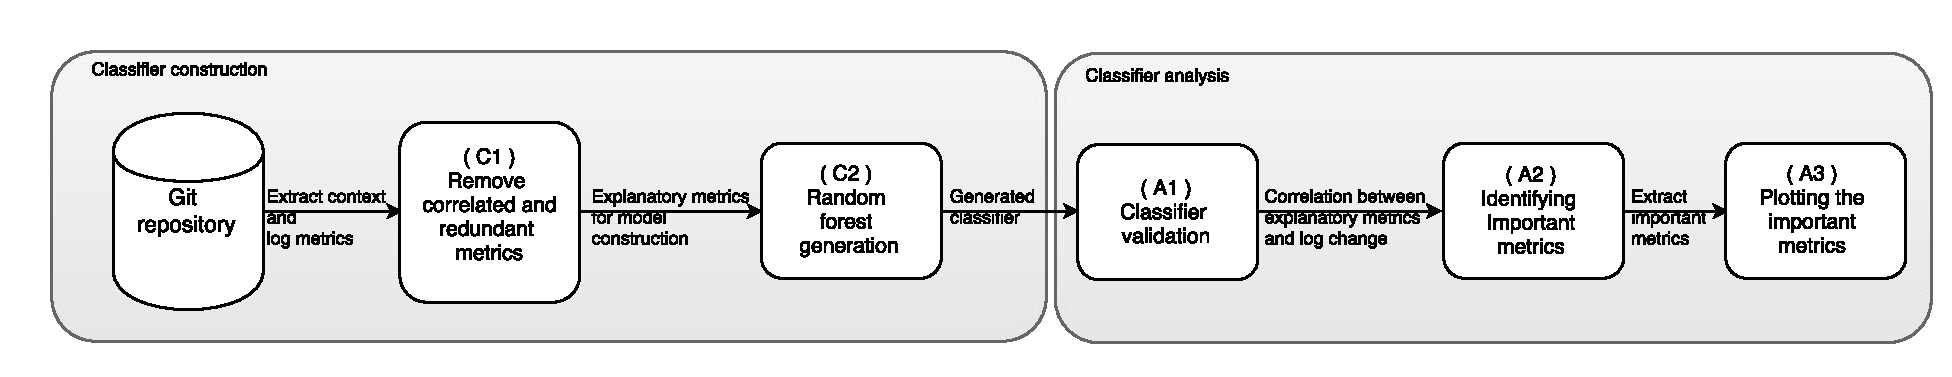
\includegraphics[width=1\columnwidth]{ModelCreationLogGeanology}
	\caption{Overview of Model construction(C) and Evaluation}
	\label{fig:ModelCreationLogGeanology}
\end{figure}  




\begin{figure}
	\centering
	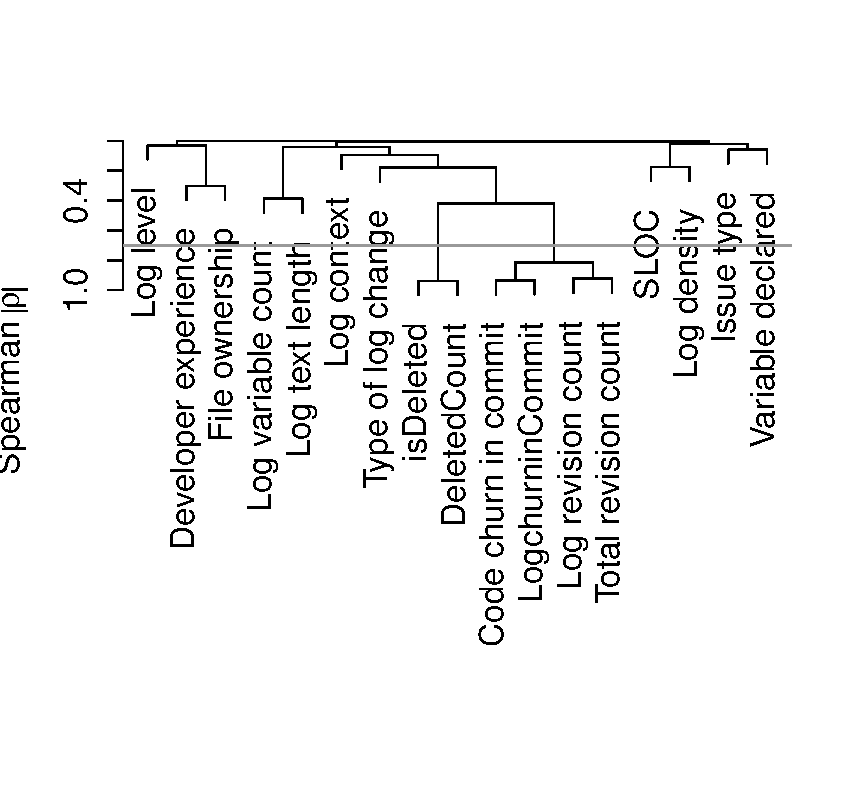
\includegraphics[height=1\columnwidth,width=0.9\columnwidth]{SpearmanActiveMQ}
 \vspace*{-1cm}	\caption{Hierarchical clustering of variables according to Spearman’s $\rho$ in ActiveMQ}
	\label{fig:SpearmanActiveMQ}
\end{figure}


\textbf{\noindent\textsl{(C2 - Random forest generation)}}

After we eliminate the correlated metrics from our datasets, we construct the random forest model.`Random forest' is a black-box ensemble classifier, which operates by constructing a multitude of decision trees on the training set and uses this to classify the testing set.
\begin{figure}
	\centering
	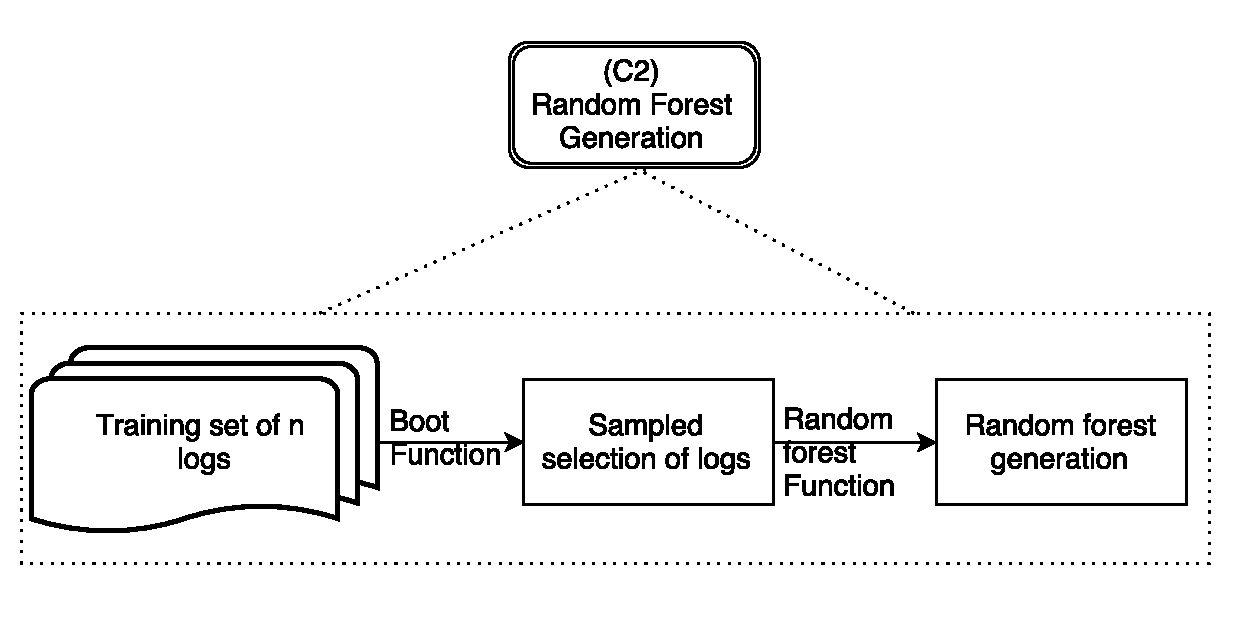
\includegraphics[height=.7\columnwidth,width=1\columnwidth]{BootRandomForest}
	\caption{ Overview of random forest generation in C2}
	\label{fig:BootRF}
\end{figure}


Given a dataset of \textsl{n} logs for training, $ D = \{ (X_{1}Y_{1},...,(X_{n}Y_{n}) \} $ where $X_{i}, i = 1...n$, is a vector of descriptors (i.e, explanatory metrics) and $Y_{i}$ is the flag which indicates whether a log is changed or not, the algorithm follows these steps and is shown in Figure~\ref{fig:BootRF}.
\begin{enumerate}
\item From the training set of \textsl{n} logs, a random sample of \emph{n} components is selected with replacement (i.e., bootstrap sample)~\cite{ShaneOLS}.

We use the `boot' function from the `boot' package in R to generate bootstrap samples. The boot function generates a set of random indices, with replacement from the integers 1:\emph{n}.

\item From the sampled selection, a tree is grown with one difference compared to normal decision trees. The random forest is split at each node using the best among subset of predictors, rather than all. This strategy helps to make the random forests more robust against over-fitting~\cite{breiman1996bagging}.

 We use the `randomForest' function from the `randomForest' package in R to generate the random forest model. 


\item The above steps are repeated until \textsl{M} such models are grown.
\item Predict new data by aggregating the prediction of the $M$ models generated.
\end{enumerate}  

\begin{table}[t]
\centering
	\begin{tabular}{|>{\raggedright}p{0.1\columnwidth}>{\raggedright}p{0.2\columnwidth}|l>{\raggedright}p{0.2\columnwidth}|}
		\hline 
		\multicolumn{1}{|>{\raggedright}p{0.03\columnwidth}}{\multirow{2}{0.03\columnwidth}{}} &  & \multicolumn{2}{c|}{Predicted}\tabularnewline
		&  & Log has changed & Log has not-changed\tabularnewline
		\hline 
		\multirow{2}{0.03\columnwidth}{Actual} & Log has changed  & TP (True Positive)  & FN (False Negative ) \tabularnewline
		& Log has not-Changed  & FP (False Positive )  & TN (True Negative) \tabularnewline
		\hline 
	\end{tabular}\protect\caption{Confusion Matrix}
	
	
	\label{tba:ConfusionMatrix} 
\end{table}

\textbf{
\noindent \textsl{(C3 - Model evaluation)}}

After we build the random forest model, we evaluate the performance of our model using precision, recall, F-measure and Brier Score. All these measures are functions of the confusion matrix as shown in Table~\ref{tba:ConfusionMatrix} and are explained below.

\textsl{Precision (P)} measure the correctness of our model in predicting which log will undergo a change in the future. It is defined as the number of logs which were accurately predicted as changed over all logs predicted to have changed as explained in Equation~\ref{f:precision}.   \\
	 \begin{equation}
 P =  \dfrac{TP}{TP + FP } 
 \label{f:precision}
	 \end{equation}	
	 
\textsl{Recall (R)} measure the completeness of our model. A model is said to be complete if the model can predict all the logs which will get changed in our dataset. It is defined as the number of logs which were accurately predicted as changed over all logs which actually change as explained in Equation~\ref{f:recall}.
	 \begin{equation}
	 R =  \dfrac{TP}{TP + FN } 
	 \label{f:recall}
	 \end{equation}	
	 
\textsl{F-Measure} is the harmonic mean of precision and recall, combining the inversely related measure into a single descriptive statistic as shown in Equation~\ref{f:Fmeasure}~\cite{F-Measure}.
	 \begin{equation}
	 F =  \dfrac{2 \times P \times R}{P + R } 
	 \label{f:Fmeasure}
	 \end{equation}	
	 
\textsl{Brier Score (BS)} is a measure of the accuracy of the predictions in our model. It is the mean squared error of the probability forecasts~\cite{wilks2011statistical}. The most common formulation of Brier Score is shown in Equation~\ref{f:BS}, where $f_{t}$ is the probability that was predicted, $o_{t}$ is the actual outcome of the event at the instance $t$ (0 if log is not changed and 1 if it is changed), and $N$ is the number of forecasting instances. 

If the predicted value is 70\% and the log is changed, the Brier Score is 0.09 (lower the Brier score, the more likely the event will occur). It reaches 0.25 for random guessing (i.e., predicted value is 50\%) and it is 0 when predicted value is 100\% and the log is not changed. 

	 \begin{equation}
	 BS =  \dfrac{1}{N}\Sigma_{t=1}^{N} (f_{t} - o_{t} )^{2} 
	 \label{f:BS}
	 \end{equation}	

The model performance measure, described previously only provide insight into how the random forest models fit the observed dataset, but it may overestimate the performance of the model if it is over-fit. We take performance overestimation (i.e., \textsl{optimism} ) into account by by subtracting the bootstrap averaged optimism~\cite{ShaneOLS} from the initial performance measure. The \textsl{optimism} of the performance measures are calculated as follows:
\begin{enumerate}
	\item From the original dataset with \textsl{n} records, select a bootstrap sample with \textsl{n} components with replacement.
	\item Build random forest using the bootstrap sample.
	\item Apply the model built from bootstrap data on both the bootstrap and original data sample, calculating precision, recall, F-measure and Brier score for both data samples.
	\item Calculate \textsl{Optimism} by subtracting the performance measures of the bootstrap sample against the original sample. 	
\end{enumerate}

	The above process is repeated 1,000 times and the average (mean) \textsl{optimism} is calculated. Finally, we calculate \textsl{optimism-reduced} performance measures for precision, recall, F-measure and Brier score by subtracting the averaged optimism of each measure, from their corresponding original measure.  The smaller the optimism values, the more stable that the original model fit is.
	\\

\textbf{\noindent \textsl{(C4 - Importance of each metric in relation to log stability)}}
To find the importance of each metric in a random forest model, we use a permutation test. In this test, the model built using the bootstrap data (i.e., two thirds of the original data) is applied to the test data(i.e., remaining one third of the original data).  

Then, the values of the $X_{i}$th metric of which we want to find importance for, are randomly permuted in the test dataset and the accuracy of the model is recomputed. The decrease in accuracy as a result of this permutation is averaged over all trees, and is used as a measure of the importance of metric $X_{i}$th in the random forest.

We use the `importance' function defined in `RandomForest' package of R, to calculate the importance of each metric. We call the `importance' function each time during the bootstrapping process to obtain 1000 importance scores for each metric in our dataset. 	

As we obtain 1000 data sets for each metric because of bootstrapping process, we use the \textbf{Scott-Knott} clustering to group the metric based on their means~\cite{Cluster1,Cluster2}. This is done to group metrics which are strong predictors of likelihood of log change. The SK algorithm uses the hierarchical clustering approach to divide the metrics and uses the likelihood ratio test to judge the difference between the groups. This assures the means of metrics within a group not to be statistically significantly different. We use the `SK' function in the `ScottKnott' package of R and set significance threshold of 0.05 to cluster the metrics into different groups. 
%\begin{table}

%	\centering

\begin{figure}[tb]
	
	\centering
	\subfloat{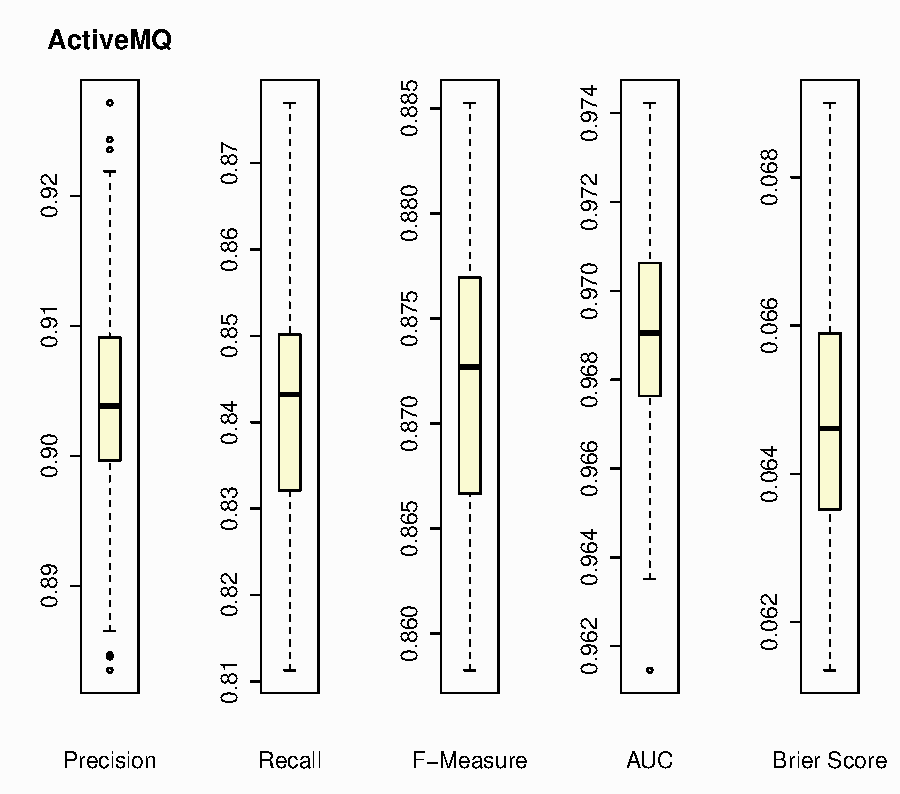
\includegraphics[width=0.49\columnwidth]{ActiveMQResults}\label{fig:f4}}
	\hfill
	\centering
	\subfloat{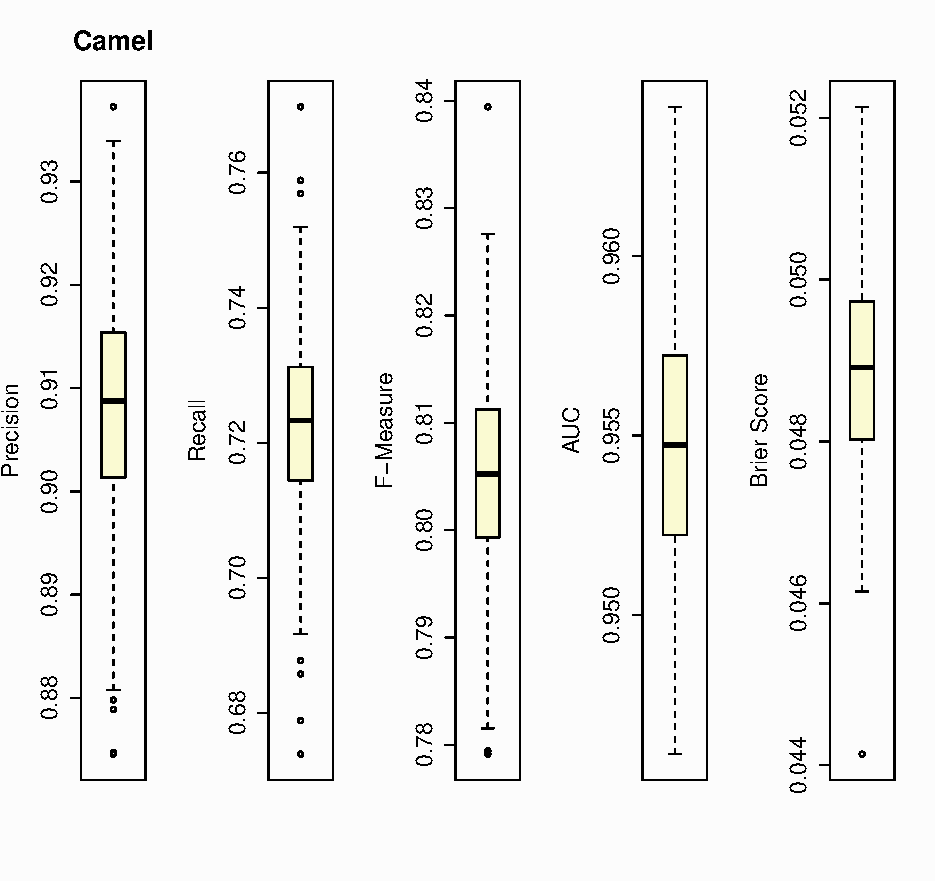
\includegraphics[width=0.49\columnwidth]{CamelResults} }
	\hfill
		\centering
		\subfloat{\includegraphics[width=0.49\columnwidth]{CloudStackResults}
			\label{fig:f4}}
		\hfill
			\centering
			\subfloat{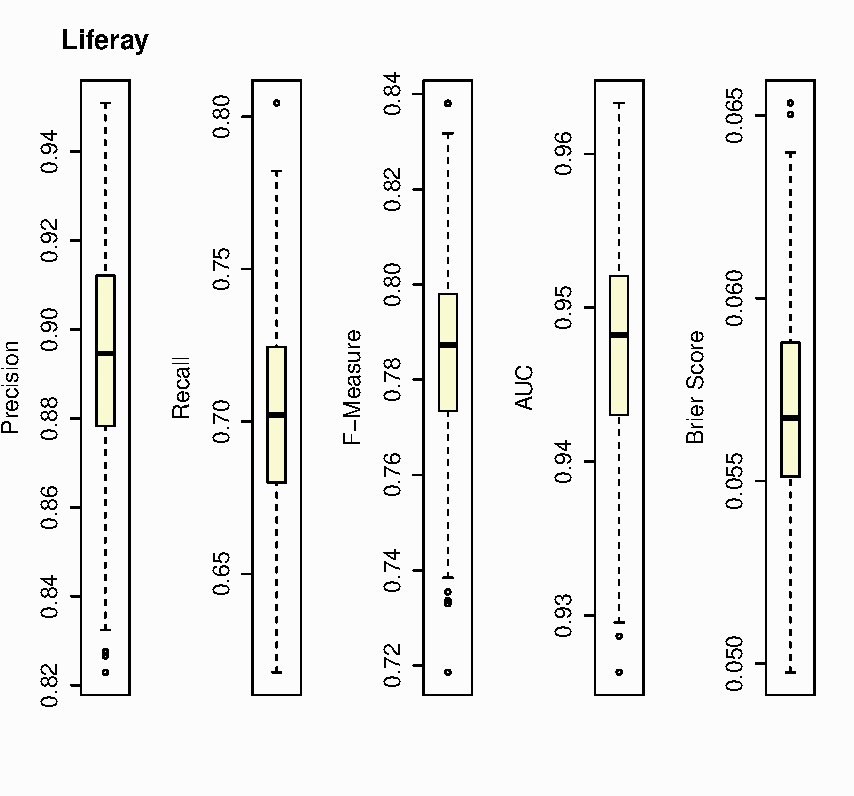
\includegraphics[width=0.49\columnwidth]{LiferayResults}\label{fig:f4}}
			\hfill
%	\caption{Distribution of the number of developers responsible for changing a log}
		\caption{The optimism reduced performance measures of the four projects}
	\label{fig:optmisim}

\end{figure}


%\label{tba:optmisim}
%\end{table}


\noindent \textbf{Results}

\textbf{The random forest classifier achieves a precision of 0.89-0.91 and recall of 0.71-0.91 for our studied systems.} Figure~\ref{fig:optmisim} shows the optimism-reduced values of	\textsl{precision}, \emph{recall}, \emph{F-measure} and \emph{Brier score} for each project. We find the recall for random forest classier in Liferay is not as high as the other projects. This may be because Liferay has the lowest percentage of logs which are changed at 20\%, compared to 45-70\% in the other projects. Because of the lower percentage of logs which are changed, the random forest classifier has fewer nodes (trees) and likelihood of false negatives is higher. 

\textbf{The random forest classifier outperforms random guessing.} The classifier achieves Brier scores between 0.04 and 0.07 across all projects. As the Brier score measure the total difference between the event and the forecast probability of the event, a perfect classifier  will have Brier score of 0 and perfect misfit classifier will have Brier score of 1 (predicts probability of log change when log not changed). This means lower the Brier score value, the better our random forest classifier. 

\subsubsection*{\textbf{Important metrics for log stability}}


From Table~\ref{tba:Scott} we see that `file ownership', `SLOC', `log density', and `developer experience' are common across all the projects in our studied systems. 
%The high importance of \emph{SLOC}, \emph{code churn in commit} and \emph{\# of comments} indicate that log stability 

%% LyX 2.1.2 created this file.  For more info, see http://www.lyx.org/.
%% Do not edit unless you really know what you are doing.
\begin{table*}[t]
	\protect\protect\caption{The important values of the metrics (top 8), divided into homogeneous
		groups by Scott-Knott clustering. The `+' sign signify positive
		correlation of the metric on log stability i.e., increase in metric increases the likelhood of log change and vice-versa.  }
	\centering
		\begin{tabular}{|lll|lll|}
			\hline 
			& \textbf{ Active MQ}  &  &  & \textbf{CloudStack}  & \tabularnewline
			\hline 
			\textbf{Rank}  & \textbf{Factors}  & \textbf{Importance}  & \textbf{Rank}  & \textbf{Factors}  & \textbf{Importance} \tabularnewline
			\hline 
			1  & SLOC & 0.174 +  & 1  & Code churn in commit & 0.138 + \tabularnewline
			2  & File ownership   & 0.162 +  & 2 & File ownership  & 0.136 + \tabularnewline
			& Log variable count & 0.161 +  &  & Developer experience & 0.135 - \tabularnewline
			3 & Developer experience & 0.140 +  & 3  & Log density  & 0.122 - \tabularnewline
			4  & Log density & 0.120 -  & 4  & SLOC & 0.122 + \tabularnewline
			5  & Variable Declared  & 0.090 -  & 5  & Log variable count & 0.113 + \tabularnewline
			6  & Deleted count & 0.082 -  & 6  & Log text length & 0.102 + \tabularnewline
			7  & Log level & 0.078 -  & 7  & Variable Declared  & 0.076 + \tabularnewline
			8  & Log churn in commit & 0.060 +  & 8  & Type of log change & 0.063 + \tabularnewline
			\hline 
		\end{tabular} \\	
			\centering	
		\begin{tabular}{|lll|lll|}
			\hline 
			& \textbf{Life Ray}  &  &  & \textbf{Camel}  & \tabularnewline
			\hline 
			\hline 
			\textbf{Rank}  & \textbf{Factors}  & \textbf{Importance}  & \textbf{Rank}  & \textbf{Factors}  & \textbf{Importance} \tabularnewline
			\hline 
			1  & Log density  & 0.152 -  & 1  & File ownership  & 0.207 + \tabularnewline
			2  & File ownership  & 0.137 -  & 2  & Log density  & 0.175 - \tabularnewline
			& Developer experience & 0.137 +  &   & Developer experience & 0.174 - \tabularnewline
			3 & SLOC & 0.127 +  & 3  & SLOC & 0.168 + \tabularnewline
			4  & Issue Id & 0.096 -  & 4 & Log variable count & 0.124 + \tabularnewline
			5  & Variable Declared  & 0.093 +  & 5  & Log level & 0.116 - \tabularnewline
			& Log variable count & 0.091 +  & 6  & Elapsed time & 0.109 - \tabularnewline
			6  & Log level & 0.081 -  &   & Issue type & 0.108 + \tabularnewline
			7 & Elapsed time & 0.072 + &   & Variable Declared  & 0.108 + \tabularnewline
			\hline 
		\end{tabular} \label{tba:Scott} 
	\end{table*}



We find that \emph{log density} and \emph{log variable count} are important metrics in our studied systems as shown in Table~\ref{tba:Scott}. We find that log density has negative correlation in all the studied systems. This suggests that when source code is well logged i.e., more logs per lines of code, the logs may communicate the necessary information making them more stable. Whereas, in files with fewer logs per lines of code, the logs have to be changed more to convey the necessary information.  We also find \emph{log variable count} has a positive correlation, implying that more text in a log results in a higher likelihood that a log will be changed. This may be because there are inconsistencies between logs and the actual needed information intended as shown by prior research~\cite{Characterizinglogs} and developers have to update logs to resolve the inconsistencies.


We find that \emph{SLOC}(source lines of code), \emph{Variable declared} are strong predictors of log change across all projects. \emph{SLOC}  has positive correlation suggesting that logs in larger files have higher likelihood of getting changed. We find that \emph{Variable declared} has positive correlation in three of the studied systems, which suggests that when developers add new variables in the commit there is a higher likelihood of log change as they may add or modify the log to output the new data.
%, logs around those comments are less likely to get changed. 


We find that \emph{file ownership} is a strong predict of log change and has positive correlation in three of the studied systems. This suggests that logs introduced by developers who have little ownership are more unstable and have to be changed. This is seen RQ1 Figure~\ref{fig:ChangedvsUnchangedlogs}, where in in three of the studied systems, the logs which change are introduced by developers who have lower ownership of a file. 

We find that \emph{developer experience} is also a strong predictor of log change in all our models but the correlation is split within the projects. We find that in Cloudstack and Camel, developer experience has negative correlation on log change, where as in ActiveMQ and Liferay developer experience has positive correlation. The positive correlation may be because of strong code ownership seen ActiveMQ and liferay where two developer are responsible for over 50\% of the total commits within the projects. 

%We find that positive correlation might be due strong code ownership in ActiveMQ and Liferay where two developers are responsible for over 50\% of the total commits, within these projects. The negative effect in ActiveMQ and Cloudstack suggests that logs written by more experienced developers are less likely to be changed. 



% This suggests that either (1) more experienced developers have logged the file increasing the stability of the logs or (2) less experienced developers have logged the file making logs unstable. 
%
%In these systems we find that, more logs are introduced by developers with less experience than developers greater experience. 


%This may be because (1) logs that are added by less experience developers are less stable or (2) more experienced developers might not be as careful about logging as new developers.

 

%
% This implies that logs introduced by more experienced developers and are more likely to be changed.  This may be because the experienced developers may be more complacent than less experienced developers, who thoroughly log the code. 

%We find that other metrics from the developer dimension are not consistent among the studied systems. This may be because each project might have different philosophy of development, for example we find that \emph{resolution time} has negative effect in Liferay and Camel but has positive effect in ActiveMQ. This suggests that logs are more likely to change in ActiveMQ when the resolution time of issue increases, but less likely in Liferay and Camel. 


\hypobox {Our Random Forest classifier achieves a precision of0.89-0.91 and recall of 0.71-0.91 across all studied systems. We find file ownership, SLOC, developer experience and log density to be strong predictors of log change in our studied systems.}










\section{Related Work}
\label{related}

In this section, we present prior empirical research done on logs and tools developed to assist in logging.

%in which log behavior in software applications is analyzed. In addition, we discuss tools developed to assist in logging. 

\subsection{Log Tools}


%Much of the prior work leverages logs for detecting anomalies in large scale systems. Lou {et al}$.$~\cite{JGLouMining} propose an approach to use the variable values printed in logs to detect anomalies in large systems. Similarly, Fu {et al}$ . $~\cite{QFuanomaly} built a finite state automaton using unstructured logs to detect performance bugs in distributed systems. In debugging, Yuan {et al$.$}~\cite{Yuan:2010:SED:1736020.1736038} propose an approach to automatically infer the failure scenarios when a log is printed during a failed run of a system.
%
%
%Logs are leveraged during load testing of large scale systems. The data collected from logs during load tests helps developers diagnose faults in the system. Jiang {et al$ . $}~\cite{Jiang:2008:AAA:1400155.1400158,JiangICSM2008,JiangICSM20092,Jiang:2010:ICS:1850000.1850068} proposed log analysis approaches to assist in automatically verifying results from load tests. Their log analysis approaches first automatically abstract logs into system events~\cite{Jiang:2008:AAA:1400155.1400158}. Based on the such events, they identified both functional anomalies~\cite{JiangICSM2008} and performance degradations~\cite{JiangICSM20092} in load test results.


Tan {et al}$ . $~\cite{TanSalsa} propose a tool named SALSA, which constructs state-machines from logs. The state-machines are further used to detect anomalies in distributed computing platforms. Yuan {et al$ . $}~\cite{Yuan} show that logs need to be improved by providing additional . Their tool named \emph{Log Enhancer} can automatically provide additional control and data flow parameters into the logs thereby improving the logs. \emph{Log Enhancer} can improve the quality of log added and mitigate the need for changes later. However, it does not provide any insight into why some logging statements are more likely to be changed. Our paper, tries to classify which logging statements have higher likelihood of being changed later and avoid such logging statements from the analysis. 
%tools assist developers to improve logging so developers can log the right information when the log is introduced


% show that output logs are leveraged for various activities such as debugging, anomaly detection, load test analysis and diagnose faults. However, when logging statements are changed, the output logs leveraged by these tools and analysis can change. These changes in the output logs, can break the tools and leads to erroneous results in the analysis.

% Based on the variable values in logs, their approach creates invariants (e.g., equations). Any new logs that violates the invariant are considered to be a sign of anomalies. Fu {et al}$ . $~\cite{QFuanomaly} built a finite state automaton using unstructured logs to detect performance bugs in distributed systems.  \indent Xu {et al}$.$~\cite{ConsoleLogs} link output logs to logs in source code to recover the text and and the variable parts of logs in source code. They applied Principal Component Analysis (PCA) to detect system anomalies. To assist in fixing bugs using logs, Yuan {et al$.$}~\cite{Yuan:2010:SED:1736020.1736038} propose an approach to automatically infer the failure scenarios when a log is printed during a failed run of a system.
%
%

%Logs are leveraged during load testing of large scale systems. The data collected from logs during load tests helps developers diagnose faults in the system. Jiang {et al$ . $}~\cite{Jiang:2008:AAA:1400155.1400158,JiangICSM2008,JiangICSM20092,Jiang:2010:ICS:1850000.1850068} proposed log analysis approaches to assist in automatically verifying results from load tests. Their log analysis approaches first automatically abstract logs into system events~\cite{Jiang:2008:AAA:1400155.1400158}. Based on the such events, they identified both functional anomalies~\cite{JiangICSM2008} and performance degradations~\cite{JiangICSM20092} in load test results. The extensive prior research on log analysis shows that logs are leveraged for different purposes and changing logs can affect the performance of log analysis tools. 


%and changes to logs can affect performance  of log analysis tools. 

% In addition, they proposed an approach that leverage logs to reduce the load test that are performed in user environment~\cite{Jiang:2010:ICS:1850000.1850068}. Shang {et al$.$}~\cite{IanContextinformation} propose an approach to leverage logs in verifying the deployment of Big Data Analytics applications. Their approach analyzes logs in order to find differences between running in a small testing environment and a large field environment.
%
%
%Logs are also leveraged in debugging software systems. Jiang {et al}$.$~\cite{Jiang:2009:UCP:1525908.1525912} study the leverage of logs in troubleshooting issues from storage systems. They find that logs assist in a faster resolution of issues in storage systems. Beschastnikh \textsl{et al}$ . $~\cite{Beschastnikh:2011:LEI:2025113.2025151} designed automated tools that infers execution models from logs. These models can be used by developers to understand the behaviors of concurrent systems. Moreover, the models also assist in verifying the correctness of the system and fixing bugs.
%\subsection {Log Tools}


%While these works focus more on enhancing existing logs in the system, our paper focuses more on informing developers which logs are more likely to get changed and identifying which factors explain the change of logs. 


%As a first step, we study how many logs are stable and how many undergo changes across commits. Our findings show that more 20-80\% of the logs are changed at-least once and 3-11\% of the logs are changed frequently. 


\subsection{Empirical Studies on Logging statements}


Prior research performs an empirical study on the characteristics of logging statements. Yuan et al.~\cite{Characterizinglogs} study the logging characteristics in four open source systems. They find that over 33\% of all changes to logging statements are after-thoughts and that logging statements are changed 1.8 times more often than regular code. Fu {et al$.$}~\cite{Fu1} performed an empirical study on where developers put logging statements. They find that logging statements are used for assertion checks, return value checks, exceptions, logic-branching and observing key points. The results of the analysis were evaluated by professionals from the industry and an F-measure of over 95\% was achieved. 


%empirical studies on logs, show that 1) logging statements are changed by developers for various reasons 2) changes to logging stateme


%and there are many contributing factors for the change. This motivates our study as we find that logs are changed for different reasons. It also helps in 

%In our work, we use the intuitions and characteristics to collect relevant context and log metrics, to correctly classify the likelihood of log change.   

Research also shows that logs are a source of information about the execution of large software systems for developers and end users. Shang et al. performed an empirical study on the evolution of both static logs and logs outputted during run time~\cite{EMSEIAN,PaperIanCIIII}. They find that logging statements are co-evolving with software systems. However, logging statements are often modified by developers without considering the needs of operators which even affects the log processing tools which run on top of the logs produced by these statements. They highlight the fact that there is a gap between operators and developers of software systems, especially in the leverage of logs~\cite{IanGap}. Furthermore, Shang et al.~\cite{IanIcesm} find that understanding logs is challenging. They examine user mailing lists from three large open-source projects and find that users of these systems have various issues in understanding logs outputted by the system. 


The existing empirical studies on logging statements show that 1) logs are leveraged by developers for different purposes and 2) logging statements are changed extensively by developers without consideration of other stakeholders,  which affect practitioners and end users. These findings highlight the need for better understanding of the stability of logging statements in the applications. 

%motivate the need for understanding the stability of logging statements in applications, which is not done by any prior studies to our best knowledge. 



  
% This gap between developers and system operators can be avoided if the logging statements leverage 

% research works highlight that developers and system operators leverage logs and changing logging statements can affect both.

%. Our work tries to tackle this problem by identifying logs which are more likely to change in the early stages so developers and system operators so they can be made more stable.  


\section{Threats to Validity}
\label{threats}
In this section, we present the threats to the validity to our findings. \\


\noindent \textbf{External Validity}

Our empirical study is performed on Liferay, ActiveMQ, Camel and CloudStack. Though these studied applications have years of history and large user bases, these applications are all Java-based. Other languages may not use logs as extensively. Our projects are all open source and we do not verify the results on any commercial platform applications. More studies on other domains and commercial platforms, with other programming languages are needed to see whether our findings can be generalized. 



\noindent \textbf{Construct Validity}


Our heuristics to extract logging source code may not be able to extract every log in the source code. Even though the studied applications-leverage logging libraries to generate logs at runtime, there may still exist user-defined logs. By manually examining the source code, we believe that we extract most of the logs. Evaluation on the coverage of our extracted logs can address this threat.


%We use keywords to identify bug fixing commits when the JIRA issue ID is not included in the commit messages. Although such keywords are used extensively in prior research~\cite{EMSEIAN}, we may still fail to identify bug fixing commits or branching and merging commits.

We use Levenshtein ratio and choose a threshold to identify modifications to logs. However, this threshold may not accurately identify modifications to logs. Further sensitivity analysis on this threshold is needed to better understand the impact of the threshold to our findings. \\

%Our models are incomplete, i.e., we have not measured all potential dimensions that impact logging stability like file and log ownership metrics, code complexity measures. However, we feel that our metrics are good and additional new dimensions can compliment our dimension to improve the explanation.\\ 

\noindent \textbf{Internal Validity}

Our study is based on the data obtained from Git for all the studied applications. The quality of the data contained in the repositories can impact the internal validity of our study.

Our analysis of the relationship between metrics that are important factors in predicting the stability of logs cannot claim causal effects, as we are investigating correlation and not causation. The important factors from our random forest models only indicate that there exists a relationship which should be studied in depth in future studies. 





\section{Conclusion}
\label{conc}
Logging statements are snippets of code, added by developers to yield valuable information about the execution of an application. Logging statements generate their output in logs, which are used by a plethora of log processing tools to assist in software testing, performance monitoring and system state comprehension. These log processing tools are completely dependent on the logs and hence are affected when logging statements are changed.

In order to reduce the effort required for the maintenance of log processing tools, we examine changes made to logging statements in four open source applications. The goal of our work is to help developers of log processing tools decide whether a logging statement is likely to change in the future. We consider our work an important first step towards helping developers to build more robust log processing tools, as knowing whether a log will change in the future allows developers to let their log processing tools rely on logs generated by logging statements that are likely to remain unchanged. The highlights of our work are:

%In this paper we study the stability of logs using a random forest classifier. The classifier is used to predict which logs are more likely to change in the future using context and log data.  The highlights of our study are:

\begin{itemize}
	\item We find that 20\%-40\%  of logs are changed at-least once.
	\item Our random forest classifier for predicting whether a log will change achieves a precision of 83\%-91\% and recall of 65\%-85\%. 
	\item Logging statements added by very experienced developer are less likely to be changed.
	\item Logging statements added by a developer who owns more than 75\% of a file, is less likely to be changed. 
	\item We find that log density, SLOC, developer experience, file ownership are important predictors of log stability in the studied applications.  	
%	\item We find that log density has negative correlation in all projects which suggests that when source code is well logged i.e., more logs per lines of code, the logs convey the needed information and are more stable. 
	
%	We find a negative correlation between developer experience and log changes from the developer dimension. We find that the number of comments in source code, also has negative correlation towards log changes. 
\end{itemize}

Our findings highlight that we can correctly classify the likelihood of a log change when log is added into the application. The important metrics from the classifier help in determining the likelihood of a log change, and developers can use this knowledge to be more selective when importing logging statements into their processing tools. 

% which logs have a higher likelihood of getting changed when they are introduced. This information can be used by system administrators and practitioners, to identify logs which have a higher chance of affecting the log processing tools and prevent failure of these tools.  






%\begin{acknowledgements}
%If you'd like to thank anyone, place your comments here
%and remove the percent signs.
%\end{acknowledgements}

% BibTeX users please use one of
%\bibliographystyle{spbasic}      % basic style, author-year citations
%\bibliographystyle{spmpsci}      % mathematics and physical sciences
%\bibliographystyle{spphys}       % APS-like style for physics
%\bibliography{}   % name your BibTeX data base

% Non-BibTeX users please use
\bibliographystyle{IEEEtran}
\bibliography{Logreference}

\end{document}
% end of file template.tex

